\documentclass[a4paper,11pt]{article}
\pdfoutput=1 % if your are submitting a pdflatex (i.e. if you have
             % images in pdf, png or jpg format)

\usepackage{jheppub} % for details on the use of the package, please
                     % see the JHEP-author-manual

\usepackage[T1]{fontenc} % if needed
\usepackage[table]{xcolor}
%\usepackage[dvipsnames]{xcolor}
\usepackage{graphicx}
\usepackage{url}
\usepackage{hyperref}
\usepackage{enumitem}
\usepackage{booktabs}
\usepackage{rotating}
%\usepackage[dvipsnames]{xcolor}
%\usepackage{natbib}
%\usepackage{biblatex}
%\addbibresource{machinebib.bib}


\definecolor{light-gray}{gray}{0.95}
\newcommand{\code}[1]{\colorbox{light-gray}{\texttt{#1}}}
\newcommand{\codewhite}[1]{\colorbox{white}{\texttt{#1}}}




%%\title{\boldmath A title with some math: $x=1$}


\title{Machine Learning for Survival Analysis: A New Approach}


%% %simple case: 2 authors, same institution
\author{D. Dooling}
\author{P. Green}
\author{A. Kim}
\author{D. Scroggin}
\author{L. Stevens}
\author{J. Webster}
%% \author{and A. Nother Author}
\affiliation{Innovative Oncology Business Solutions, \\
  4901 Lang Ave NE, \\
 Albuquerque, NM 87109, USA}
%% \affiliation{Institution,\\Address, Country}

% more complex case: 4 authors, 3 institutions, 2 footnotes
%\author[a,b,1]{F. Irst,\note{Corresponding author.}}
%\author[c]{S. Econd,}
%\author[a,2]{T. Hird\note{Also at Some University.}}
%\author[a,2]{and Fourth}

% The "\note" macro will give a warning: "Ignoring empty anchor..."
% you can safely ignore it.

%\affiliation[a]{One University,\\some-street, Country}
%\affiliation[b]{Another University,\\different-address, Country}
%\affiliation[c]{A School for Advanced Studies,\\some-location, Country}

% e-mail addresses: one for each author, in the same order as the authors
\emailAdd{ddooling@innovativeobs.com}
\emailAdd{pgreen@innovativeobs.com}
\emailAdd{akim@innovativeobs.com}
\emailAdd{dscroggin@innovativeobs.com}
\emailAdd{lstevens@innovativeobs.com}
\emailAdd{jwebster@innovativeobs.com}







\abstract{We have applied a little-known data transformation on subsets of the Surveillance, 
Epidemiology, and End Results (SEER) publically available data of the National Cancer 
Institute (NCI) to make it suitable input to standard machine learning classifiers. This transformation properly treats the right-censored data in the SEER data and the resulting Random Forest and Multi-Layer Perceptron models predict full survival curves. Treating the 6, 12, and 60 months points of the resulting survival curves as 3 binary classifiers, the 18 resulting classifiers have AUC values ranging from  .765 to .885. Further evidence that the models have generalized well from the training data is provided by the extremely high levels of agreement between the random forest and neural network models predictions on the 6, 12, and 60 month binary classifiers.}



\begin{document} 
\maketitle
\flushbottom

\section{Introduction and Background}
\label{sec:intro}



Extracting actionable information from data is changing the fabric of modern business. A class of techniques that transforms data into actionable information goes by the name of Machine Learning \cite{pythonmachinelearning}.
Machine Learning has recently become a popular method to answer questions and solve problems that are too complex to solve via traditional methods. 
The Surveillance, Epidemiolgy, and End Results (SEER) Program of the National Cancer Institute (NCI) has been collecting data because intuitively researchers feel confident that this data is capturing information that has buried within it useful information in the form of  relationships between the types of data collected (demographic as well as staging information) and the survival outcomes.
Though this relationship evades capture by traditional methods, it is possible to surface it with the two machine learning techniques known as \textbf{Random Forests} and \textbf{Neural Networks}. These two methods produce very similar results when applied to the SEER dataset, and are based on two almost diametrically opposed learning philosophies, which lends confidence in the validity of the results.

The Surveillance, Epidemiolgy, and End Results (SEER) Program of the National Cancer Institute (NCI) is the most recognized authoritative source of information on cancer incidence and survival in the United States. SEER currently collects and publishes cancer incidence and survival data from population-based cancer registries covering approximately 28 percent of the US population.

Quoting directly from the SEER
website \citep{seerwebsite}:

\begin{quote}
The SEER program registries routinely collect data on patient demographics, primary tumor site, tumor morphology and stage at diagnosis, first course of treatment, and follow-up for vital status. This program is the only comprehensive source of population-based information in the United States that includes stage of cancer at the time of diagnosis and patient survival data. The mortality data reported by SEER are provided by the National Center for Health Statistics. The population data used in calculating cancer rates is obtained periodically from the Census Bureau. Updated annually and provided as a public service in print and electronic formats, SEER data are used by thousands of researchers, clinicians, public health officials, legislators, policymakers, community groups, and the public.
\end{quote}





One characterstic of the SEER data and that is shared by many datasets in the medical field 
goes by the name of "censored data.'' The SEER data contains the number of months each patient survived, as well as an indicator variable showing whether or not the patient is still alive at the end of the data collection period.
Methods to deal effectively with this kind of "right-censored data'' include Kaplan-Meier curves
and Cox's Proportional Hazard models \cite{cam}. The Kaplan-Meier techniques only give estimates for cohorts of patients and are not applicable for predicting the surival curve for a single patient, and the Cox Proportional Hazard models require a fairly restrictive set ot assumptions to be satisifed in order to yield reliable results. In addition, the Cox Proportional Hazard models are not able to capture the nonlinear relationships between the given data fields that go into making predictions; they can only capture the first-order linear relationships.

Previous work applying machine learning methods to subsets of the SEER data include creative attempts to deal with the problems presented by  "right-censored data." The authors of ~\cite{ISI:000337467400005} use semi-supervised learning techniques to predict 5 year survival, essentially imputing values for SEER records where the survival months infomation is censored at a value less than 5 years. The authors of ~\cite{ISI:000355882700012} investigate the effects of comordbidities; i.e., patients with two different cancer diagnosises, but their treatment of the censored data underestimates the survival probabilities. All records representing patients who survived at least 60 months as well as all those who died earlier than 60 months were considered, but patients alive prior to 60 months but censored out of the study before 60 months were not included. This treatment biases the data and the predictions, leading to overly pessimistic survival probablilites predicted by the trained models.

To overcome these limitations of the traditional methods, IOBS has applied a little-known technique to transform the SEER data to make it amenable to more powerful machine learning methods. The essential idea is to recast the problem to an appropriate discrete classification problem instead of a regression problem (predicting survival months). Treating months after diagnosis as just another discrete feature, the SEER data (or any other right-censored data) can be transformed simply so as to make predictions for the hazard function, 
 probability of dying in the next month, given that the patient has not yet died.
The full survival function can then be derived from the hazard function.
Details of this transformation can be found in this blog post \cite{kuhn}.


%For internal references use label-refs: see section~\ref{sec:intro}.
%Bibliographic citations can be done with cite: refs.~\cite{a,b,c}.
%When possible, align equations on the equal sign. The package
%\texttt{amsmath} is already loaded. See \eqref{eq:x}.
%\begin{equation}
%\label{eq:x}
%\begin{split}
%x &= 1 \,,
%\qquad
%y = 2 \,,
%\\
%z &= 3 \,.
%\end{split}
%\end{equation}
%Also, watch out for the punctuation at the end of the equations.


%If you want some equations without the tag (number), please use the available
%starred-environments. For example:
%\begin{equation*}
%x = 1
%\end{equation*}

%The amsmath package has many features. For example, you can use use
%\texttt{subequations} environment:
%\begin{subequations}\label{eq:y}
%\begin{align}
%\label{eq:y:1}
%a & = 1
%\\
%\label{eq:y:2}
%b & = 2
%\end{align}
%and it will continue to operate across the text also.
%\begin{equation}
%\label{eq:y:3}
%c = 3
%\end{equation}
%\end{subequations}
%The references will work as you'd expect: \eqref{eq:y:1},
%\eqref{eq:y:2} and \eqref{eq:y:3} are all part of \eqref{eq:y}.

%A similar solution is available for figures via the \texttt{subfigure}
%package (not loaded by default and not shown here). 
%All figures and tables should be referenced in the text and should be
%placed at the top of the page where they are first cited or in
%subsequent pages. Positioning them in the source file
%after the paragraph where you first reference them usually yield good
%results. See figure~\ref{fig:i} and table~\ref{tab:i}.

%%%%%%%%%%%%%%%%%%%%%%%%%%%%%%%%%%%%%%


%\section{Survival Analysis}


%\textbf{Survival analysis} is a way to describe how long things last. It is often used to study %human lifetimes, but it also applies to "survival'' of mechanical and electronic components, or %more generally to intervals in time before an event.

%If someone you know has been diagnosed with a life-threatening disease, you might have %seen a "5-year survival rate,'' which is the probability of surviving five years after diagnosis. %That estimate and related statistics are the result of survival analysis.


%The fundamental concept in survival analysis is the \textbf{survival curve}, $S(t)$, which is a %function that maps from a duration, $t$, to the probability of surviving longer than $t$. If you %know the distribution of durations, or "lifetimes,'' finding the survival curve is easy; it's just the %complement  of the CDF:

%\begin{equation}
%S(t) = 1 - CDF(t)
%\end{equation}

%where $CDF(t)$ is the probability of a lifetime less than or equal to $t$.
%From the survival curve we can derive the \textbf{hazard function}; for pregnancy lengths, %the 
%hazard function maps from a time, $t$, to the fraction of pregnancies that continue until $t$ %and then end at $t$. To be more precise:

%\begin{equation}
%\lambda(t) = \frac{ S(t) - S(t+1)}{S(t)}
%\end{equation}

%The numerator is the fraction of lifetimes that end at $t$, which is also $PMF(t)$.

%If someone gives you the CDF of lifetimes, it is easy to compute the survival and hazard %functoins. But in many real-world scenarios, we can't measure the distribution of lifetimes %directly. We have to infer it.

%For example, suppose you are following a group of patients to see how long they survive after %diagnosis. Not all patients are diagnosed on the same day, so at any point in time, some %patients have survived longer than others. If some patients have died, we know their survival %times. For patients who are still alive, we don't know survival times, but we have a lower %bound.

%If we wait until all patients are dead, we can compute the survival curve, but it we are %evaluating the effectiveness of a new treatment, we can't wait that long! We need a way to %estimate survival curves using incomplete information. 




%Traditionally, survival analysis was developed to measure lifespans of individuals. An actuary or %health professional would ask questions like ``how long does this population live for?'', and %answer it using survival analysis. For example, the population may be a nation’s population (for actuaries), or a population sticken by a disease (in the medical professional’s case). %Traditionally, sort of a morbid subject.

%The analysis can be further applied to not just traditional \textit{births} and 
%\textit{deaths}, but any duration. Medical professional might be interested in the time %between childbirths, where a birth in this case is the event of having a child , and a death is %becoming pregnant again! (obviously, we are loose with our definitions of birth and death) %Another example is users subscribing to a service: a birth is a user who joins the service, and %a death is when the user leaves the service.


%At the time you want to make inferences about durations, it is possible, likely true, that not all %the death events have occured yet. For example, a medical professional will not wait 50 years %for each individual in the study to pass away before investigating – he or she is interested in %the effectiveness of improving lifetimes after only a few years, or months possibly.

%The individuals in a population who have not been subject to the death event are labeled as %right-censored, i.e. we did not (or can not) view the rest of their life history due to some %external circumstances. All the information we have on these individuals are their current %lifetime durations (which is naturally less than their actual lifetimes).


%A common mistake data analysts make is choosing to ignore the right-censored individuals.
%If we naively decide to \textit{not} include the right-censored individuals, it is clear that we %would be severely underestimating the true average lifespan. Furthermore, if we instead %simply took the mean of \textit{all} observed lifespans, including the current lifespans of right-%censored instances, we would \textit{still} be underestimating the true average lifespan.


%Survival analysis was originally developed to solve this type of problem, that is, to deal with %estimation when our data is right-censored. Even in the case where all events have been %observed, i.e. no censorship, survival analysis is still a very useful to understand durations.


%We next introduce the two fundamental objects in survival analysis, the \textit{survival %function} and the \textit{hazard function}.


\section{Methodology}


\subsection{Data acquisition}

We used the publically available 1973-2012 SEER incidence data files corresponding to colon, breast and lung cancer contained in the following list.
SEER requires that researchers submit a request for the data, which includes an agreement form. Detailed documentation explaining the contents of both the incidence data files used in this study as well as a data dictionary for the 1973-2012 SEER incidence data files are available without the need to register or submit a data request \cite{seerdoc}.
 

\begin{itemize}[noitemsep]
\item incidence\symbol{92}yr1973\_2012.seer9\symbol{92}COLRECT.txt
\item incidence\symbol{92}yr1973\_2012.seer9\symbol{92}BREAST.txt
\item incidence\symbol{92}yr1973\_2012.seer9\symbol{92}RESPIR.txt
\item incidence\symbol{92}yr1992\_2012.sj\_la\_rg\_ak\symbol{92}COLRECT.txt
\item incidence\symbol{92}yr1992\_2012.sj\_la\_rg\_ak\symbol{92}BREAST.txt
\item incidence\symbol{92}yr1992\_2012.sj\_la\_rg\_ak\symbol{92}RESPIR.txt
\item incidence\symbol{92}yr2000\_2012.ca\_ky\_lo\_nj\_ga\symbol{92}COLRECT.txt
\item incidence\symbol{92}yr2000\_2012.ca\_ky\_lo\_nj\_ga\symbol{92}BREAST.txt
\item incidence\symbol{92}yr2000\_2012.ca\_ky\_lo\_nj\_ga\symbol{92}RESPIR.txt
\item incidence\symbol{92}yr2005.lo\_2nd\_half\symbol{92}COLRECT.txt
\item incidence\symbol{92}yr2005.lo\_2nd\_half\symbol{92}BREAST.txt
\item incidence\symbol{92}yr2005.lo\_2nd\_half\symbol{92}RESPIR.txt
\end{itemize}



\subsection{Data preparation and preprocessing}
\label{subsec:dataprep}

A great deal of data munging is necessary before using these SEER incidence files as input into machine learning algorithms. A preprocessing step common to each of three cancer types studied involves the \codewhite{STATE-COUNTY RECODE}.
The \codewhite{STATE-COUNTY RECODE} field is a state-county combination where the first two characters represent the state FIPS code and the last three digits represent the FIPS county code.  
This particular field illustrates an important feature of machine learning, that between \textit{categorical features} and \textit{numeric features}. All input into a machine learning algorithm must be numeric, but real numbers carry with them the usually extremely useful property known as the well-ordering property of the real numbers. But if one is tasked with encoding a categorical feature into suitable numeric format for machine learning, it is necessary to do so in a way that removes the well-ordering property~\cite{bowles}. 

As a simple example of how to correctly treat categorical variables in a mchine learning context, consider the SEER variable \codewhite{SEX}. This variable is encoded with a numeric 1 for males and a numeric 2 for females as shown in Table ~\ref{tab:sex}. Values such as "Male" and "Female" encoded as numbers are dangerous because if not handled properly, they can generate bogus results \cite{downey}. The proper way to transform the SEER \codewhite{SEX} variable is to create two additional variables: \codewhite{sex$\_$Male} and \codewhite{sex$\_$Female}, and then to eliminate the variable \codewhite{SEX}. For example,


%%\begin{displaymath}
%%\begin{table}[tbp]
%\begin{center}
%%\begin{tabular}{|c|}
%%\hline
%%$\mathbf{SEX}$ \\ \hline
%%1 \\ \hline
%%\end{tabular}
%\end{center}
%%\end{table}
%%$\rightarrow$
%%\begin{table}[tbp]
%%\begin{tabular}{|c|c|}
%\begin{center}
%\hline
%$\mathbf{sex\_Male}$ & $\mathbf{sex\_Female}$ \\ \hline
%1 & 0 \\
%\end{tabular}
%%\end{center}
%\end{table}
%\end{displaymath}



\begin{equation}
\left[ \begin{array}{l}
\mbox{SEX} \\ \hline
1 \end{array} \right]
\rightarrow 
\left[ \begin{array}{l|l}
\mbox{sex$\_$Male} & \mbox{sex$\_$Female} \\ \hline
1 & 0 \end{array} \right]
\label{eqn:onehotmale}
\end{equation}

and 

\begin{equation}
\left[ \begin{array}{l}
\mbox{SEX} \\ \hline
2 \end{array} \right]
\rightarrow 
\left[ \begin{array}{l|l}
\mbox{sex$\_$Male} & \mbox{sex$\_$Female} \\ \hline
0 & 1 \end{array} \right]
\label{eqn:onehotfemale}
\end{equation}




\begin{table}[tbp]
\begin{center}
\begin{tabular}{cc}
\toprule
Code & Description \\ 
\midrule
1 & Male \\  
2 & Female \\  
\bottomrule
\end{tabular}
\caption{\label{tab:sex} Encoding of gender in the SEER incidence files. These types of categorical variables need to be transformed via one-hot-encoding.}
\end{center}
\end{table}


The procedure outlined in Equations~(\ref{eqn:onehotmale},~\ref{eqn:onehotfemale}) needs to be applied to all of the nominal categorical variables in the SEER data that we wish to include in our predictive models.
In particular, in order to include the geophgraphical information contained in the SEER categorical variable \codewhite{STATE-COUNTY RECODE}, it becomes necessary to create a new feature variable for each of the distinct (state,county) pairs in the data. In the United States, there are approximately 3,000 counties. Clearly, transforming the \codewhite{STATE-COUNTY RECODE} data representation into distinct (state$\_$county) columns will explode the data to become wider than is optimal for machine learning. Adding extra columns to your dataset, making it wider, requires more data rows (making it taller) in order for machine learning algorithms to effectively learn~\cite{bowles}. Because one-hot coding \codewhite{STATE-COUNTY RECODE} would cause such drastic shape changes in our data, we wish to avoid doing so. Fortunately, this variable, though given as a categorical variable, is actually an ordinal variable. There is an ordering among the (state$\_$county) columns, name longitude, latitude, and elevation. We can transform the data in \codewhite{STATE-COUNTY RECODE} into three new numerical columns: \codewhite{lat}, \codewhite{lng}, and \codewhite{elevation}.

For example, Table~(\ref{tab:nmhead}) shows how five entries of \code{STATE-COUNTY RECODE} corresponding to counties within New Mexico would can be represented by the 
\code{elevation}, \code{lat}, and \code{lng} features.

\begin{table}[tbp]
\begin{center}
\begin{tabular}{llrrr}
\toprule
 STATE-COUNTY RECODE &               address &    elevation &        lat &         lng \\
\midrule
35001 &  Bernalillo+county+NM &  5207.579772 &  35.017785 & -106.629130 \\
35003 &      Catron+county+NM &  8089.242628 &  34.151517 & -108.427605 \\
35005 &      Chaves+county+NM &  3559.931671 &  33.475739 & -104.472330 \\
35006 &      Cibola+county+NM &  6443.415570 &  35.094756 & -107.858387 \\
35007 &      Colfax+county+NM &  6147.749089 &  36.579976 & -104.472330 \\
\bottomrule
\end{tabular}
\caption{\label{tab:nmhead} Example of the transformation of \code{STATE-COUNTY RECODE} to \code{elevation}, \code{lat}, and \code{lng}.}
\end{center}
\end{table}

It is a simple exercise to construct the full lookup table from the SEER \\  \code{STATE-COUNTY RECODE} variable to the corresponding three values \code{elevation}, \code{lat}, and \code{lng}. Using the publically available dafafile from the United States Census Bureau~\cite{census} to construct query strings like the values of the \code{address} field in Table (~\ref{tab:nmhead}), it is possible to then programmatically query the Google Maps Geocoding API for the latitude and longitude~\cite{geocode}, and the Google Maps Elevation API for the corresponding elevation~\cite{elevation}.
An added benefit of this shift from the single categorical variable \code{STATE-COUNTY RECODE} to the three continuous numerical variables \code{lat}, \code{lng}, and \code{elevation} is that input into the web applications described later are not restricted to the states and counties covereed in the SEER registries. The full lookup table analogous to Table~\ref{tab:nmhead} is available from a GitHub repository containing supplemental information for this study~\cite{supp}.


\subsection{Colon Cancer Data}
\label{subsec:coloncancerdata}

In this section we describe the data processing steps that were specific to the colon cancer model development. The four COLRECT.txt files were imported into a pandas DataFrame object.
This data was then filtered according to the conditions in Table~\ref{tab:colonfilter}.






\begin{table}[tbp]
\begin{center}
\begin{tabular}{lr}
\toprule
 Column &  Filter \\
\midrule
\codewhite{SEQUENCE NUMBER-CENTRAL} & \codewhite{$\neq$ "Unspecified"} \\
\codewhite{AGE AT DIAGNOSIS} & \codewhite{$\neq$ "Unknown age"} \\
\codewhite{BIRTHDATE-YEAR} & \codewhite{$\neq$ "Unknown year of birth"} \\
\codewhite{YEAR OF DIAGNOSIS} & \codewhite{$\geq 2004$} \\
\codewhite{SURVIVAL MONTHS FLAG} & \codewhite{= "1"}\\
\codewhite{CS TUMOR SIZE EXT/EVAL} & \codewhite{$\neq$ ""} \\
\codewhite{CS TUMOR SIZE} & \codewhite{$\neq 999$} \\
\codewhite{SEER RECORD NUMBER} & \codewhite{$= 1$} \\
\codewhite{PRIMARY SITE} & \codewhite{ $=$ "LARGE INTESTINE, (EXCL. APPENDIX)"} \\
\codewhite{SEQUENCE NUMBER-CENTRAL} & \codewhite{$=0$} \\
\bottomrule
\end{tabular}
\caption{\label{tab:colonfilter} Filters applied to the Colon Cancer data.}
\end{center}
\end{table}






The following categorical features were one-hot encoded as described in 
section~\ref{subsec:dataprep}:

\begin{itemize}[noitemsep]
\item \codewhite{SEX},
\item  \codewhite{MARITAL STATUS AT DX},
\item \codewhite{RACE/ETHNICITY},
\item \codewhite{SPANISH/HISPANIC ORIGIN},
\item \codewhite{GRADE},
\item \codewhite{PRIMARY SITE},
\item \codewhite{LATERALITY},
\item \codewhite{SEER HISTORIC STAGE A},
\item \codewhite{HISTOLOGY RECODE--BROAD GROUPINGS},
\item \codewhite{MONTH OF DIAGNOSIS},
\item  \codewhite{VITAL STATUS RECODE}.
\end{itemize}
The \codewhite{STATE-COUNTY RECODE} variable was dropped and replaced with the \codewhite{elevation}, \codewhite{lat}, and \codewhite{lng} variables as illustrated in Table~\ref{tab:nmhead}.

With just the above data preparation, it is possible to construct traditional Kaplan-Meier estimates of the survival curves for the colon cancer population represented by this subset of the data.
After the above one-hot encoding procedure, the new variable
\codewhite{vital\_status\_recode\_Dead} indicates that the patient is deceased if this variable = 1, or else that the patient's record is right-censored if this variable = 0.
\codewhite{SURVIVAL MONTHS} and \codewhite{vital\_status\_recode\_Dead} are all that is needed to construct the Kaplan-Meier estimate shown in Figure~(\ref{fig:colonkaplan}).




\begin{figure}[tbp]
\centering 
%\begin{center}/\end{center} takes some additional vertical space
%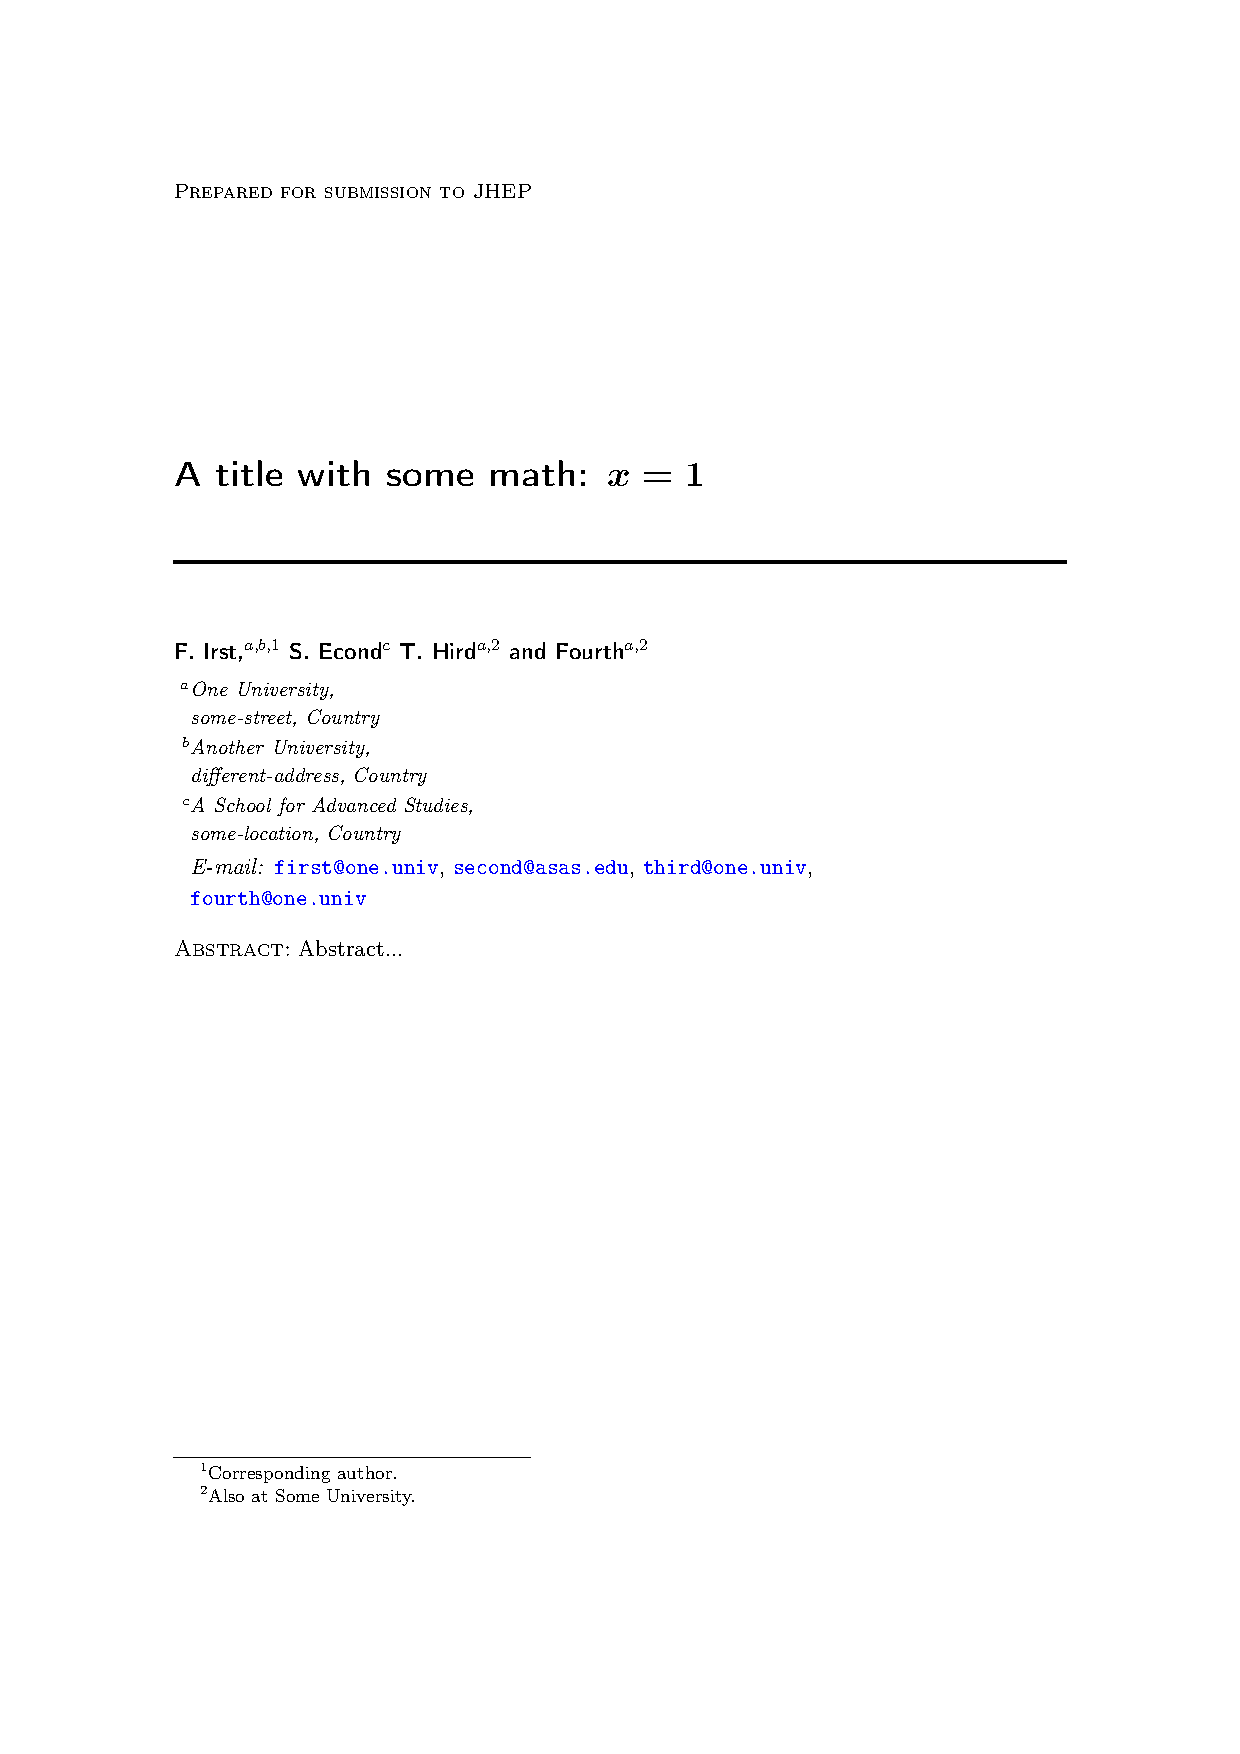
\includegraphics[width=.45\textwidth,trim=0 380 0 200,clip]{img1.pdf}
%\hfill
\begin{center}
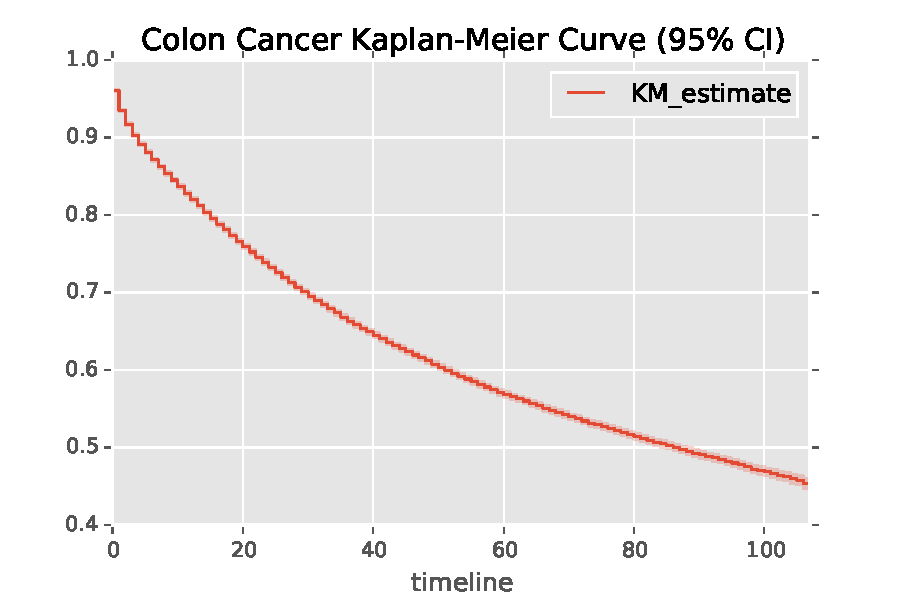
\includegraphics[width=.90\textwidth,origin=c]{colonkaplan.pdf}
% "\includegraphics" is very powerful; the graphicx package is already loaded
\caption{\label{fig:colonkaplan} Traditional Kaplan-Meier estimate of the survival curve for all colon cancer patients. Fitted with 113072 observations, 71804 censored.}
\end{center}
\end{figure}





\subsection{Lung Cancer Data}
\label{subsec:lungcancerdata}

In this section we describe the data processing steps that were specific to the lung cancer model development. The four RESPIR.txt files were imported into a pandas DataFrame object.
This data was then filtered according to the conditions in Table~\ref{tab:lungfilter}.
The same list of categorical features as in the colon cancer case were then one-hot encoded.



\begin{table}[tbp]
\begin{center}
\begin{tabular}{lr}
\toprule
 Column &  Filter \\
\midrule
\codewhite{SEQUENCE NUMBER-CENTRAL} & \codewhite{$\neq$ "Unspecified"} \\
\codewhite{AGE AT DIAGNOSIS} & \codewhite{$\neq$ "Unknown age"} \\
\codewhite{BIRTHDATE-YEAR} & \codewhite{$\neq$ "Unknown year of birth"} \\
\codewhite{YEAR OF DIAGNOSIS} & \codewhite{$\geq 2004$} \\
\codewhite{SURVIVAL MONTHS FLAG} & \codewhite{= "1"}\\
\codewhite{CS TUMOR SIZE EXT/EVAL} & \codewhite{$\neq$ ""} \\
\codewhite{CS TUMOR SIZE} & \codewhite{$\neq 999$} \\
\codewhite{SEER RECORD NUMBER} & \codewhite{$= 1$} \\
\codewhite{PRIMARY SITE} & \codewhite{ $=$ "LUNG \& BRONCHUS"} \\
\codewhite{SEQUENCE NUMBER-CENTRAL} & \codewhite{$=0$} \\
\bottomrule
\end{tabular}
\caption{\label{tab:lungfilter} Filters applied to the Lung Cancer data.}
\end{center}
\end{table}


With just the above data preparation, it is possible to construct traditional Kaplan-Meier estimates of the survival curves for the colon cancer population represented by this subset of the data.
After the above one-hot encoding procedure, the new variable
\codewhite{vital\_status\_recode\_Dead} indicates that the patient is deceased if this variable = 1, or else that the patient's record is right-censored if this variable = 0.
\codewhite{SURVIVAL MONTHS} and \codewhite{vital\_status\_recode\_Dead} are all that is needed to construct the Kaplan-Meier estimate shown in Figure~(\ref{fig:lungkaplan}).






\begin{figure}[tbp]
\centering 
%\begin{center}/\end{center} takes some additional vertical space
%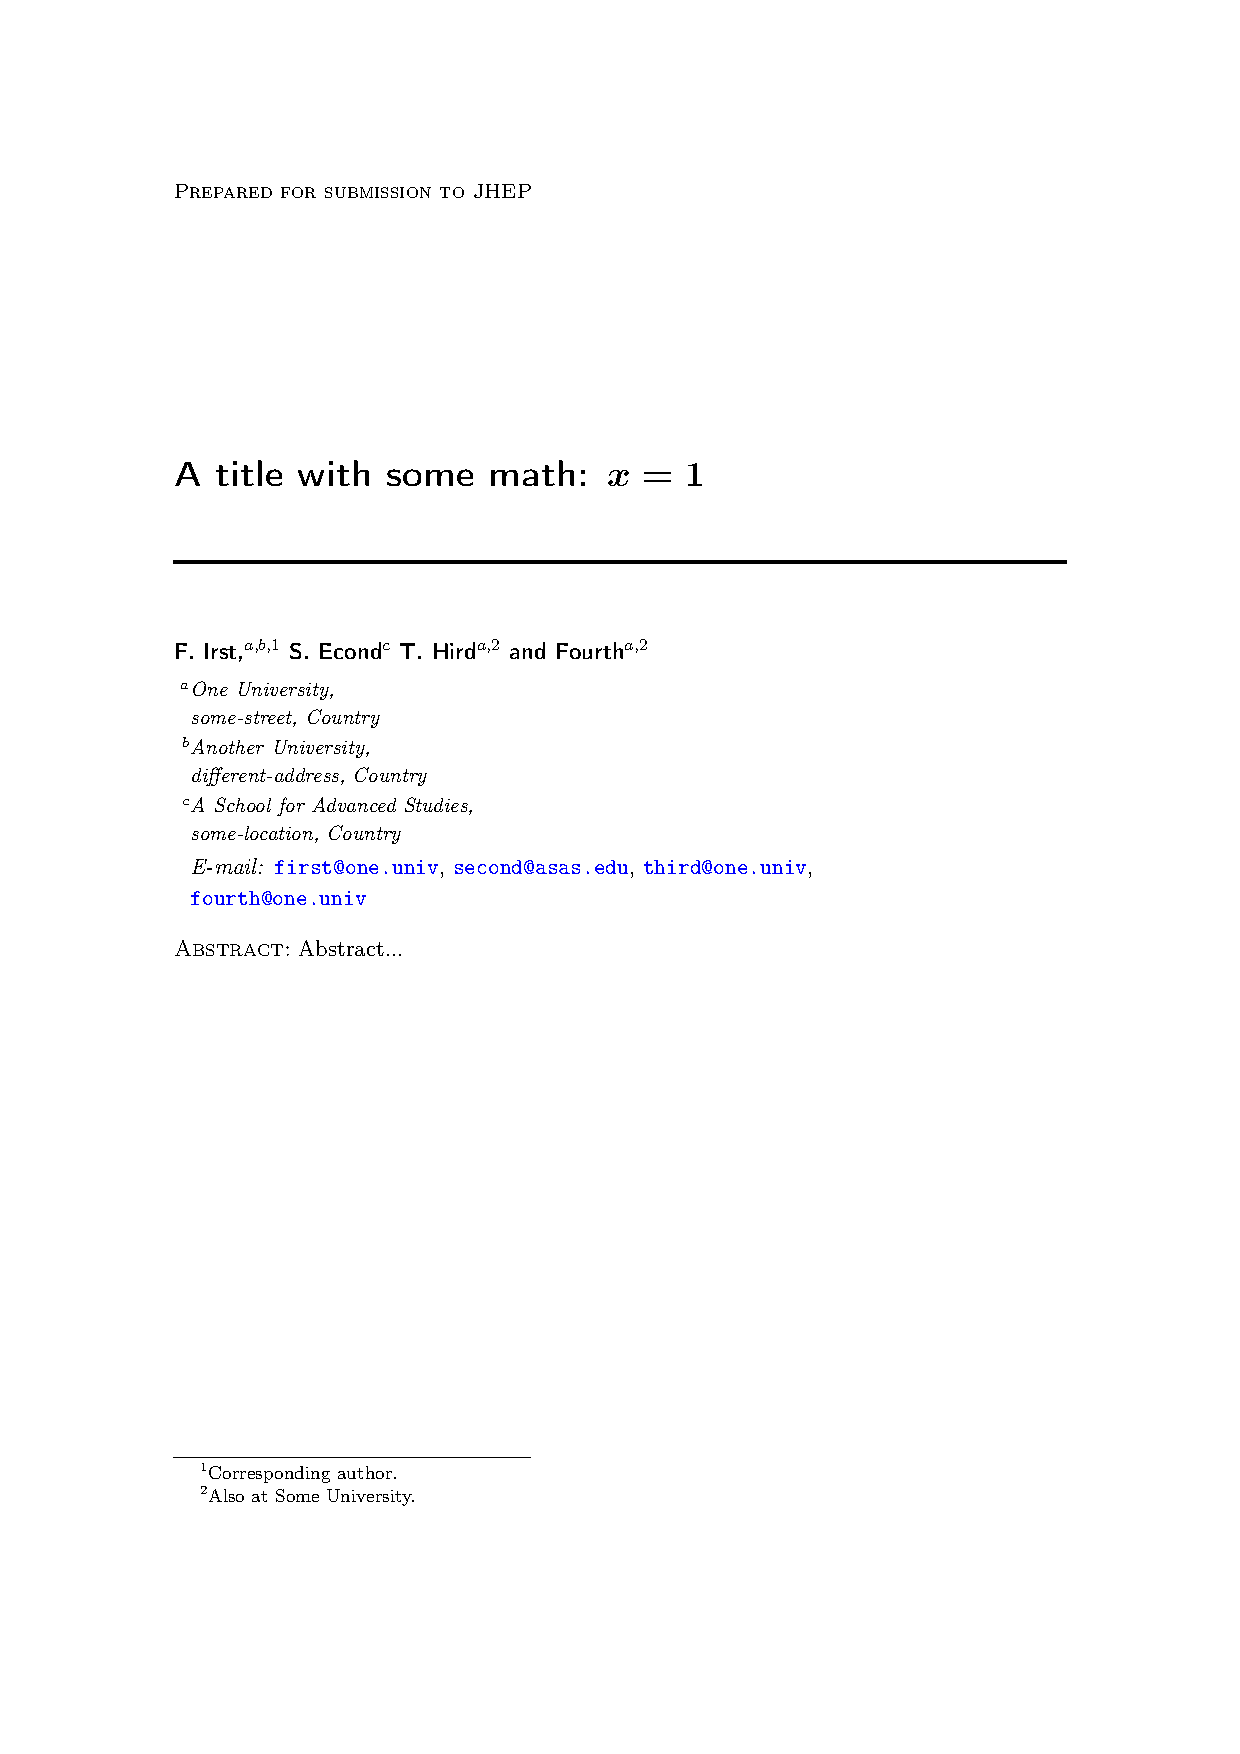
\includegraphics[width=.45\textwidth,trim=0 380 0 200,clip]{img1.pdf}
%\hfill
\begin{center}
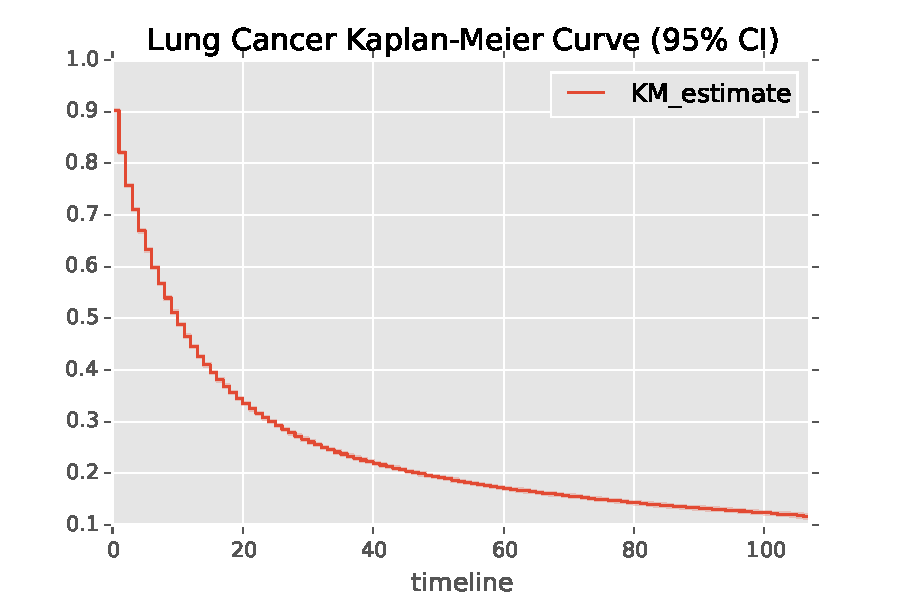
\includegraphics[width=.90\textwidth,origin=c]{lungkaplan.pdf}
% "\includegraphics" is very powerful; the graphicx package is already loaded
\caption{\label{fig:lungkaplan} Traditional Kaplan-Meier estimate of the survival curve for all lung cancer patients. Fitted with 177089 observatins, 47409 censored.}
\end{center}
\end{figure}



\subsection{Breast Cancer Data}
\label{subsec:breastcancerdata}

In this section we describe the data processing steps that were specific to the lung cancer model development. The four BREAST.txt files were imported into a pandas DataFrame object.
This data was then filtered according to the conditions in Table~\ref{tab:breastfilter}.
The same list of categorical features as in the colon cancer case were then one-hot encoded.



\begin{table}[tbp]
\begin{center}
\begin{tabular}{lr}
\toprule
 Column &  Filter \\
\midrule
\codewhite{SEQUENCE NUMBER-CENTRAL} & \codewhite{$\neq$ "Unspecified"} \\
\codewhite{AGE AT DIAGNOSIS} & \codewhite{$\neq$ "Unknown age"} \\
\codewhite{BIRTHDATE-YEAR} & \codewhite{$\neq$ "Unknown year of birth"} \\
\codewhite{YEAR OF DIAGNOSIS} & \codewhite{$\geq 2004$} \\
\codewhite{SURVIVAL MONTHS FLAG} & \codewhite{= "1"}\\
\codewhite{CS TUMOR SIZE EXT/EVAL} & \codewhite{$\neq$ " "} \\
\codewhite{CS TUMOR SIZE} & \codewhite{$\neq 999$} \\
\codewhite{SEER RECORD NUMBER} & \codewhite{$= 1$} \\
\codewhite{SEQUENCE NUMBER-CENTRAL} & \codewhite{$=0$} \\
\bottomrule
\end{tabular}
\caption{\label{tab:breastfilter} Filters applied to the Breast Cancer data.}
\end{center}
\end{table}




With just the above data preparation, it is possible to construct traditional Kaplan-Meier estimates of the survival curves for the colon cancer population represented by this subset of the data.
After the above one-hot encoding procedure, the new variable
\codewhite{vital\_status\_recode\_Dead} indicates that the patient is deceased if this variable = 1, or else that the patient's record is right-censored if this variable = 0.
\codewhite{SURVIVAL MONTHS} and \codewhite{vital\_status\_recode\_Dead} are all that is needed to construct the Kaplan-Meier estimate shown in Figure~(\ref{fig:breastkaplan}).

\begin{figure}[tbp]
\centering 
%\begin{center}/\end{center} takes some additional vertical space
%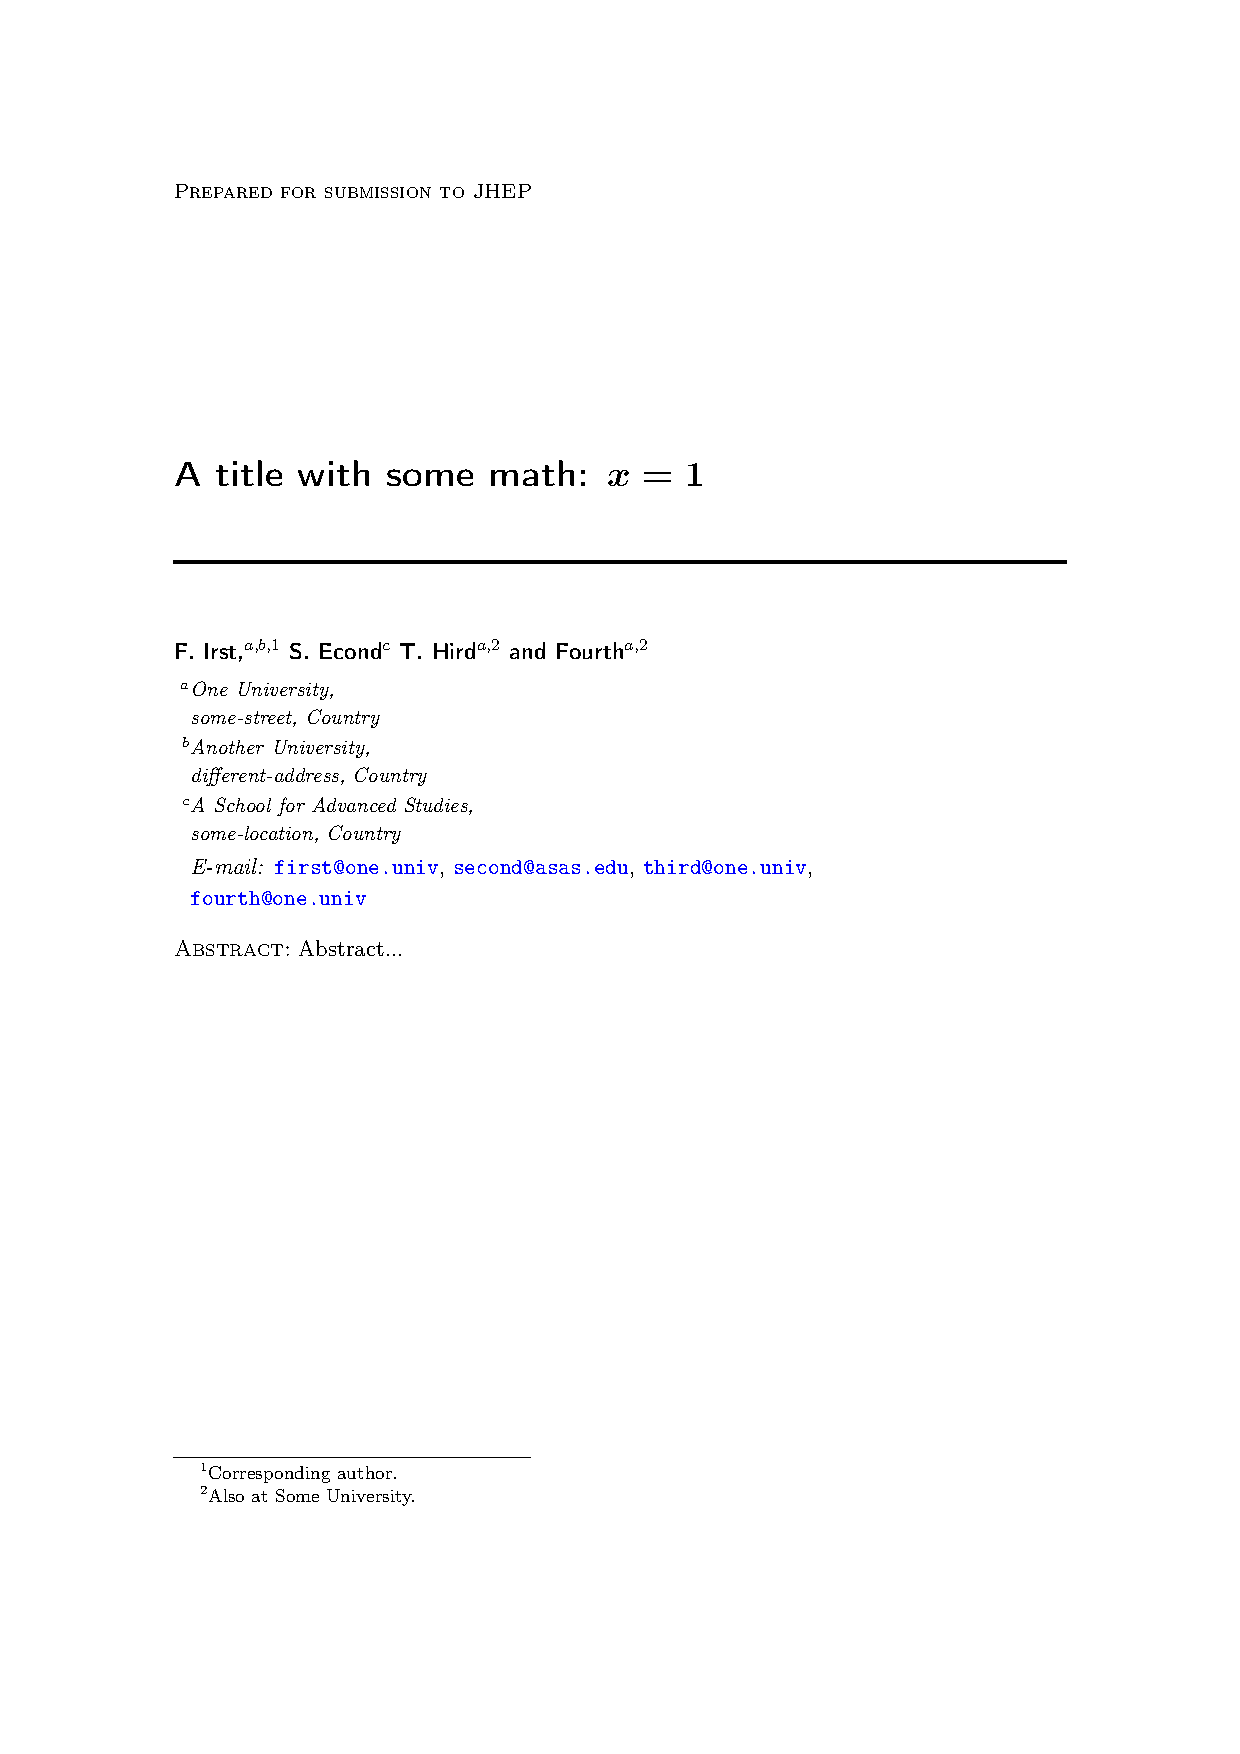
\includegraphics[width=.45\textwidth,trim=0 380 0 200,clip]{img1.pdf}
%\hfill
\begin{center}
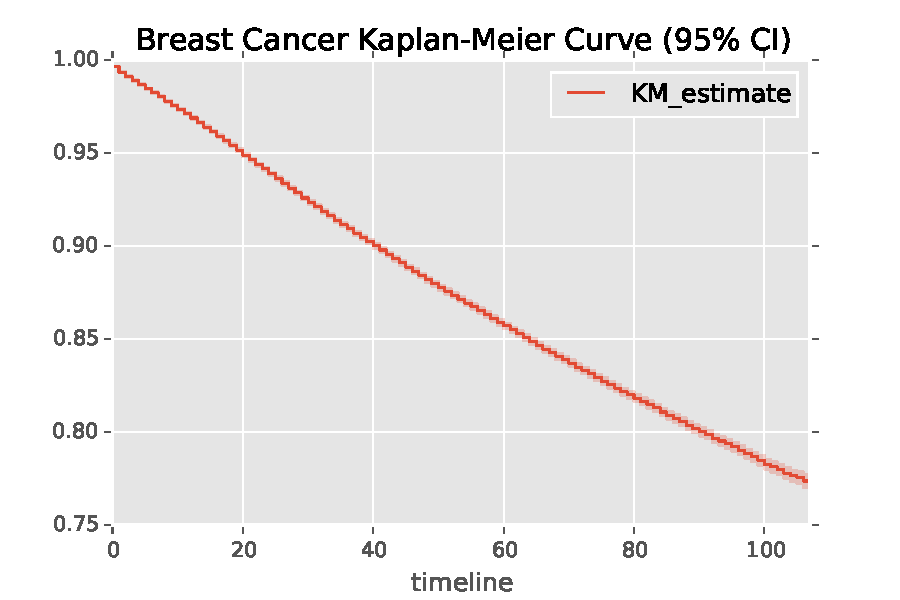
\includegraphics[width=.90\textwidth,origin=c]{breastkaplan.pdf}
% "\includegraphics" is very powerful; the graphicx package is already loaded
\caption{\label{fig:breastkaplan} Traditional Kaplan-Meier estimate of the survival curve for all breast cancer patients. Fitted with 329949 observatins, 292279 censored.}
\end{center}
\end{figure}


Before applying machine learning models trained with these data sets, we review in section~(\ref{sec:surv}) the sailent features of survival analysis and censored data. We then describe in detail a method that takes full advantage of all the data, including the right-censored data, and which involves a simple and intuitive transformation, culminating in the full set of features and target variables listed in sections~(\ref{subsec:colonfeatures},~\ref{subsec:lungfeatures},~\ref{subsec:breastfeatures}).

\section{Machine Learning Survival Analysis with Censored Data}
\label{sec:surv}


The above Kaplan-Meier estimates of the survival curves for colon (Figure~(\ref{fig:colonkaplan}), lung 
(Figure~(\ref{fig:lungkaplan}), and breast cancer (Figure~(\ref{fig:breastkaplan}) are constructed from the full population of cancer patients in the respective datasets.
An unsatisfactory consequence is that these estimates are highly course-grained, and not very meaningful to an indivual. Patients with very disparate characteristics are given the same prognosis by these Kaplan-Meier survival curve estimates. Therefore it is desirable to find robust predictors for survival curves of individual where the input is an individual record where the predictors are trained on larger populations.


% https://openaccess.leidenuniv.nl/bitstream/handle/1887/11456/01.pdf?sequence=6

\subsection{Survival Analysis}
\label{subsec:survprimer}

Survival analysis allows us to model the time until an event happens. Time-to-event measures pose unique problems for the analyst. Suppose that you want to predict the survival time for patients receiving an experimental cancer treatment. After three years, some of the patients in the study have died, and you can compute the survival time for each of these patients. However, many of the patients are still living at the end of three years; you do not know their ultimate survival time. Statisticians call this problem \textit{censoring}, a problem that surfaces when you try to model time-to-event reopnse measures using data captured over a limited time period.

The two kinds of censoring are right censoring and left censoring. If you only know that the pertinent event is 
\textit{after} some date, as is the case for patients in the preceding example who survive to the end of the study, the data is right-censored. On the other hand, if you only know that the beginning of the pertinent time-to-event took place before a certain date, the data is left-censored. For example, if you know that every patient in the study received the experimental treatment before the study started but do not know the exact date of treatment, the data is left-censored. Data can be both right-censored and left-censored.


\textit{Survival analysis} is a family of techniques developed to work with censored time-to-event response measures. Note that if censoring is not present, you may be able to model time-to-event using standard modeling techniques. For some studies, however, you would have to wait a very long time before every sampled observation has a terminal event; in the case of the experimental cancer treatment, some patients might live another 20 years. Hence, survival analysis techniques enable the analyst to take full advantage of available data without waiting until every treated patient dies, every sampled part fails, or every tracked account closes.

%\textbf{Survival analysis} is a way to describe how long things last. It is often used to study %human lifetimes, but %it also applies to "survival'' of mechanical and electronic components, or more generally to intervals in time before %an event.

%If someone you know has been diagnosed with a life-threatening disease, you might have seen a "5-year survival %rate,'' which is the probability of surviving five years after diagnosis. %That estimate and related statistics are the %result of survival analysis.


The fundamental concept in survival analysis is the \textbf{survival curve}, $S(t)$, which is a %function that maps from a duration, $t$, to the probability of surviving longer than $t$. If you know the distribution of durations, or "lifetimes,'' finding the survival curve is easy; it's just the complement  of the CDF:

\begin{equation}
\label{eq:s}
S(t) = 1 - CDF(t)
\end{equation}
where $CDF(t)$ is the probability of a lifetime less than or equal to $t$.
From the survival curve we can derive the \textbf{hazard function}; for pregnancy lengths, %the 
hazard function maps from a time, $t$, to the fraction of pregnancies that continue until $t$ %and then end at $t$. To be more precise:

\begin{equation}
\label{eq:hazard}
\lambda(t) = \frac{ S(t) - S(t+1)}{S(t)}
\end{equation}
The numerator is the fraction of lifetimes that end at $t$, which is also $PMF(t)$.
If someone gives you the CDF of lifetimes, it is easy to compute the survival and hazard functions. But in many real-world scenarios, we can't measure the distribution of lifetimes directly. We have to infer it.
For example, suppose you are following a group of patients to see how long they survive after diagnosis. Not all patients are diagnosed on the same day, so at any point in time, some patients have survived longer than others. If some patients have died, we know their survival %times. For patients who are still alive, we don't know survival times, but we have a lower bound.

If we wait until all patients are dead, we can compute the survival curve, but it we are evaluating the effectiveness of a new treatment, we can't wait that long! We need a way to %estimate survival curves using incomplete information. 




\section{Prediction Models}


\subsection{Decision Trees and Random Forests}

\begin{sidewaysfigure}[tbp]
\centering 
%\begin{center}/\end{center} takes some additional vertical space
%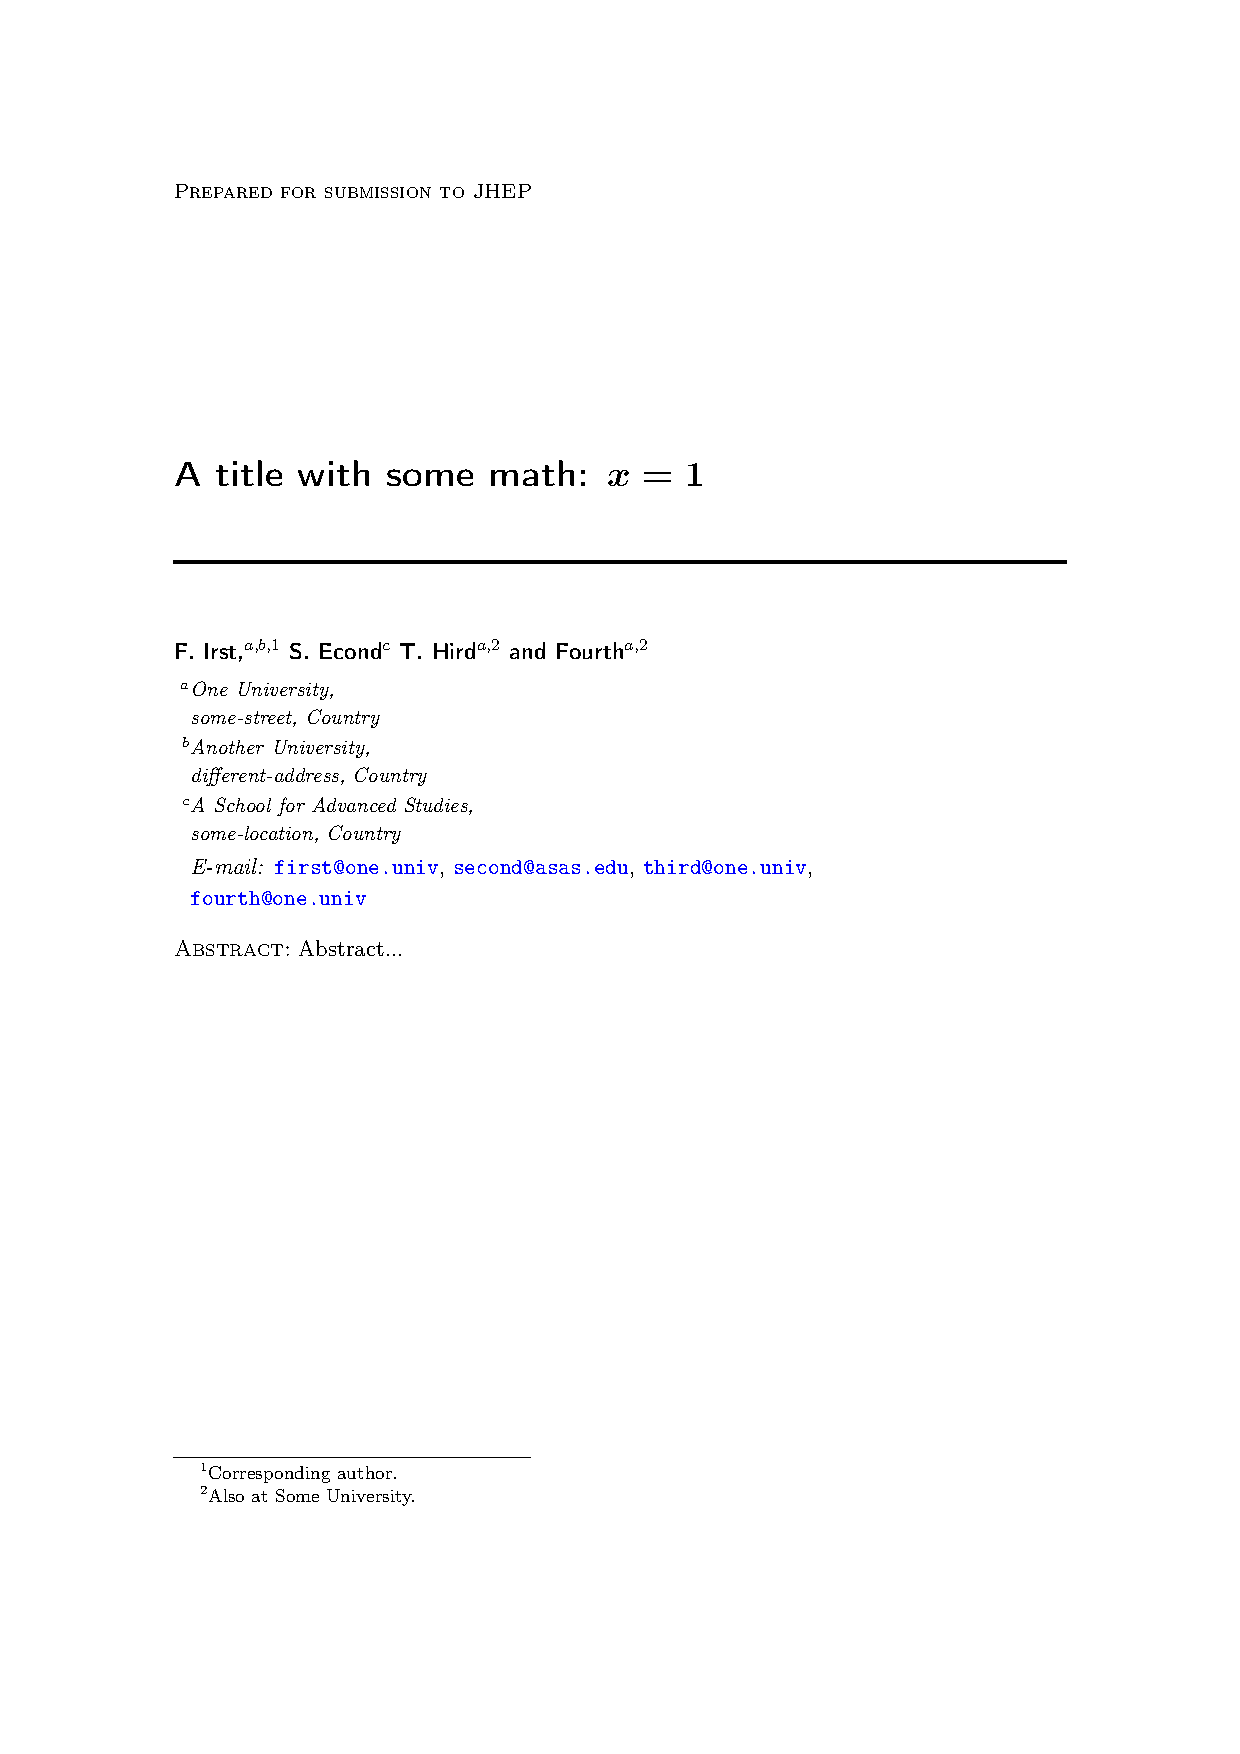
\includegraphics[width=.45\textwidth,trim=0 380 0 200,clip]{img1.pdf}
%\hfill
\begin{center}
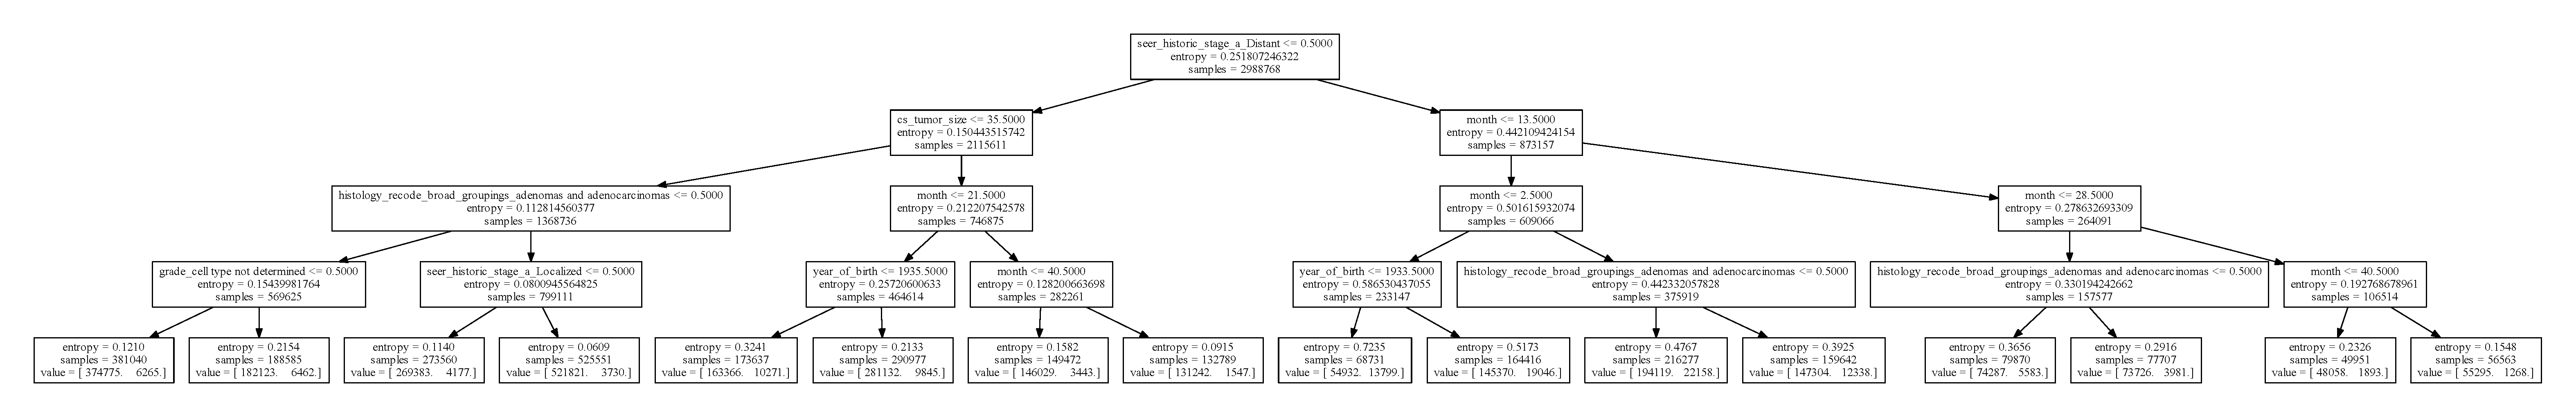
\includegraphics[width=.95\textwidth,origin=c]{lungdt.pdf}
% "\includegraphics" is very powerful; the graphicx package is already loaded
\caption{\label{fig:lungdt} The top levels of a decision tree trained on the Lung Cancer training data.}
\end{center}
\end{sidewaysfigure}


\subsection{MLP Neural Networks}









%\subsection{Survival function}

%Let $T$ be a (possibly infinite, but always non-negative) random lifetime taken from the %population under study. For example, the amount of time a couple is married. Or the time it %takes a user to enter a webpage (an infinite time it they never do). The survival function, $S(t)%$, of a population is defined as


%\begin{equation}
%S(t) = \mbox{Pr}(T \ge t)
%\end{equation}



%In human language: the survival function defines the probability the death event has not %occured yet at time $t$, or equivalently, the probability of surviving until at least
% time $t$. Note the following properties of the survival function:

%\begin{enumerate}
%\item $0 \leq S(t) \leq 1$
%\item $F_{T}(t) = 1 - S(t)$, where $F_{T}(t)$ is the CDF of $T$, which implies 
%\item $S(t)$ is a non-increasing function of $t$.
%\end{enumerate}


%\subsection{Hazard curve}

%We are also interested in the probability of dying in the next instant, given we haven't expired %yet. Mathematically, that is:

%\begin{equation}
%\begin{split}\lim_{\delta t \rightarrow 0 } \; Pr( t \le T \le t + \delta t | T > t)\end{split}
%\end{equation}


%This quantity goes to 0 as $\delta t$ shrinks, so we divide this by the interval $\delta t$ (like %we might do in calculus). This defines the hazard function at time $t, \lambda(t)$:


%\begin{equation}
%\begin{split}\lambda(t) =  \lim_{\delta t \rightarrow 0 } \; \frac{Pr( t \le T \le t + \delta t | T %> t)}{\delta t}\end{split}
%\end{equation}




%It can be shown with quite elementary probability that this is equal to:

%\begin{equation}
%\lambda(t) = \frac{-S'(t)}{S(t)}
%\end{equation}


%and solving this differential equation, we get:

%\begin{equation}
%S(t) = \exp\left( -\int_0^t \lambda(z) dz \right)
%\end{equation}

%What I love about hte above equation is that it defines \textbf{all} survival functions, and %because the hazard function is arbitrary (i.e., there is no parametric form), the entire function %is non-parametric (this allows for very flexible curves). Notice that we can now speak either %about the survival function, $S(t)$, or the hazard function, $\lambda(t)$, and we can convert %back and forth quite easily. It also gives us another, albeit less useful, expression for
% $f_T(t)$: Upon differentiation and some algebra, we recover:

%\begin{equation}
%f_T(t) = \lambda(t)\exp\left( -\int_0^t \lambda(z) dz \right)
%\end{equation}

%Of course, we do not observe the true survival curve of a population. We must use the %observed data to estimate it. We also want to continue to be non-parametric, that is not %assume anything about how the survival curve looks. The \textit{best} method to recreate the %survival function non-parametrically from the data is known as the Kaplan-Meier estimate.



%To estimate the survival function, we use the Kaplan-Meier Estimate, defined as:

%\begin{equation}
%\hat{S}(t) = \prod_{t_i < t} \frac{n_i - d_i}{n_i}
%\end{equation}

%\begin{equation}
%\hat{S}(t) = \prod_{t_i \lt t} \frac{n_i - d_i}{n_i}
%\end{equation}

%where $d_{i}$ are the number of death events at time $t$ and $n_{i}$ is the number of %subjects at risk of death just prior to time $t$.


%Put in discussion about how the methods presented by us are \textbf{personalized} survival %curves. Much more interesting, pragmatic, actionable.



%\section{Decision trees for survival analysis}

%Survival analysis is an interesting problem in machine leanring, but it doesn't get nearly as %much attention as the usual classification and regression tasks, so there aren't as many tools %for it. Here I describe a nifty reduction that allows us to bring more traditional machine-%learning tools to bear on the problem. Combined with the view of decision trees as greedy %piecewise-constant loss-minimizing classifiers, it enables a number of powerful and flexible %algorithms for large-scale discrete survival analysis.

%Discrete survival analysis is motivated by problems like disease prognosis. Suppose we're %trying to predict survival times from a rare disease. We enroll some subjects who were just %diagnosed, and we check up on them monthly until they die. Then we try to predict the time %until recurrence, $\mathbf{Y}$, from data about the patient, $\mathbf{X}$.

%We could use standard regression algorithms, but there are a couple of wrinkles:

%\begin{itemize}
%\item We only know the recurrence times up to the month, because that's how often we check %up on them, so $\mathbf{Y}$ isn't actually continuous. This is where the "discrete'' part of the %name comes from. (We could porbably get the exact death rate if we tried, but that's too %complex for us right now. Plus, it'll make the analysis harder later, as we'll see.)
%\item $\mathbf{Y}$ is known to be greater than zero. Most regression algorithms don't have a %natural way to take this account.
%\item Most importantly, \textbf{we won't be able to observe a recurrence for everyone}. Some %people will be lost to follow-up. Some people will be cured. Even some of those who die might %outlast the study period. This leads to a problem called \textit{right-censored data}, where for %certain patients we know that, say, $\mathbf{Y} > 60$ (months), but we don't know the exact %value of $\mathbf{Y}$.
%\end{itemize}

%We could get around the last one by discarding all data points that don't experience a %recurrence, but this would introduce severe selection bias. CRITICIZE THAT OTHER GUYs %PAPER THAT DOES EXACTLY THIS. Plus, it would throw away of lot of information on healthy %people. So instead we'll do something more clever.

%\subsection{The Hazard Function}

%If we were doing ordinary regression, where we had observed the $\mathbf{Y}$ for each $%%\mathbf{X}$, we would try to learn a function $f(\mathbf{X}) = E(\mathbf{Y} | \mathbf{X})$ %(or sometimes some other property of the conditional distribution of $\mathbf{Y}$, like the %median). But we don't have enough information about $\mathbf{Y}$ for that to work.

%So instead of thinking in terms of $E(\mathbf{Y} | \mathbf{X})$, we'll instead think about %something more granular called the \textit{hazard function}. The hazard function is

%\begin{equation}
%h(X, t) = P(Y=t | Y \ge t, X),
%\end{equation}
%the probability that, if someone has survived up until month $t$, they will die in that month.

%In fact, leaning $h$ will tell us \textit{more} about the disease than leaning $f$, because it %will give us not only the expected survival time but the entire distribution of survival times:

%\begin{equation}
%P(Y = t|X) = h(X, t)\prod_{i=1}^{t-1} (1 - h(X, i)),
%\end{equation}
%so we can recover the entire probability mass function.


%\subsection{A Loss Function}

%So we want to learn some approximation $\hat h(X, t) \approx h(X, t)$. But how do we decide %what a good approximation is? The obvious thing to try is maximizing the expected log-%likelihood.

%The other wrinkle is that we don't actually see $\mathbf{Y}$. Instead we see some related %variables - how long each subject was in the study $(\mathbf{T})$, and whether they exited %by dying or by being censored $(\mathbf{D})$. ($\mathbf{D}$ is a Boolean variable, so 
%$\mathbf{D} = 1$ if $\mathbf{T} = \mathbf{Y}$, and $\mathbf{D} = 0$ if $\mathbf{T} < %%\mathbf{Y}$).

%We could try to evaluate the log-likelihood of the exact data we see - that is, 
%$P(T, D|X)$. But that would require us to build a model not only of the time of death but also %the time of censorship (because we'd need the likelihood of getting censored data at time $%%\mathbf{T}$). Usually the censorship distribution is a property of the data-collection %mechanism, not the underlying reality - for instance, in clinical studies it's a property of the %follow-up time. So a prediction of it probably won't generalize well to other settings.

%For that reason, instead of evaluating the likelihood of the entire data point $(\mathbf{T}, %%\mathbf{D})$, we pretend that censorship just exogenously removes some information about %$\mathbf{Y}$. So we'll split our likelihood into two pieces:
%$P(\mathbf{Y} = \mathbf{T})$ for uncensored data, and $P(\mathbf{Y} > \mathbf{T})$ for %censored data. Given this, we can write down the log-likelihood of seeing a particular datum if 
%$\hat{h}$ were correct:








%%%%%%%%%%%%%%%%%%%%%%%%%%%%%%%%%%%%

\section{Performance Metrics}
\label{sec:performancemetrics}

% NewPatientBreastML.html
% NewPatientBreastConv.html
% NewPatientColonML.html
% NewPatientColonConv.html
% NewPatientLungML.html
% NewPatientConv.html


\begin{table}[tbp]
\begin{center}
\begin{tabular}{lrrr}
\toprule
%\rowcolors{1}{white}{yellow}
%\hline
Model & 6 Months AUC & 12 Months AUC & 60 Months AUC \\ 
\midrule
Breast RF &  .846       &     .885           &  .844 \\ 
Breast NN &   .855      &     .867      &    .836 \\ 
Colon RF  &     .804          &      .806           &      .828           \\ 
Colon NN   &     .797          &          .804         &   .841  \\ 
Lung RF    &      .772               &        .796               &   .874  \\ 
Lung NN    &        .765              &        .796               &  .875  \\
\bottomrule
\end{tabular}
\caption{\label{tab:AUC} AUC values for the Random Forest and Neural Networks model
binary classifiers derived from the full survival curve predictions; see text for details.}
\end{center}
\end{table}



%\begin{table}[tbp]
%\begin{center}
%\begin{tabular}{lr}
%\toprule
% Column &  Filter \\
%\midrule
%\codewhite{SEQUENCE NUMBER-CENTRAL} & \codewhite{$\neq$ "Unspecified"} \\
%\codewhite{AGE AT DIAGNOSIS} & \codewhite{$\neq$ "Unknown age"} \\
%\codewhite{BIRTHDATE-YEAR} & \codewhite{$\neq$ "Unknown year of birth"} \\
%\codewhite{YEAR OF DIAGNOSIS} & \codewhite{$\geq 2004$} \\
%\codewhite{SURVIVAL MONTHS FLAG} & \codewhite{= "1"}\\
%\codewhite{CS TUMOR SIZE EXT/EVAL} & \codewhite{$\neq$ " "} \\
%\codewhite{CS TUMOR SIZE} & \codewhite{$\neq 999$} \\
%\codewhite{SEER RECORD NUMBER} & \codewhite{$= 1$} \\
%\codewhite{SEQUENCE NUMBER-CENTRAL} & \codewhite{$=0$} \\
%\bottomrule
%\end{tabular}
%\caption{\label{tab:breastfilter} Filters applied to the Breast Cancer data.}
%\end{center}
%\end{table}





\subsection{Model Agreement}

TO DO: Check if comorbidites are contributing to the outliers in the agreement boxplots that follow.
Could mesh with the prevous work~\cite{ISI:000355882700012}.


\begin{table}[tbp]
\begin{center}
\begin{tabular}{lrrr}
\toprule
%\rowcolors{1}{white}{yellow}
Cancer Type & $\%$ agreement 6 months & $\%$ agreement 12 months & $\%$ agreement 60 months \\ 
\midrule
Colon & .981 & .971 & .915 \\  
Breast & .994 & .984 & .938 \\  
Lung & .861 & .883 & .900 \\  
\bottomrule
\end{tabular}
\caption{\label{tab:agree} Percentage agreement for the Random Forest and Neural Network classifiers for 6, 12, and 60 month survival predictions on the test data for each cancer type.}
\end{center}
\end{table}

\begin{figure}[tbp]
\centering 
%\begin{center}/\end{center} takes some additional vertical space
%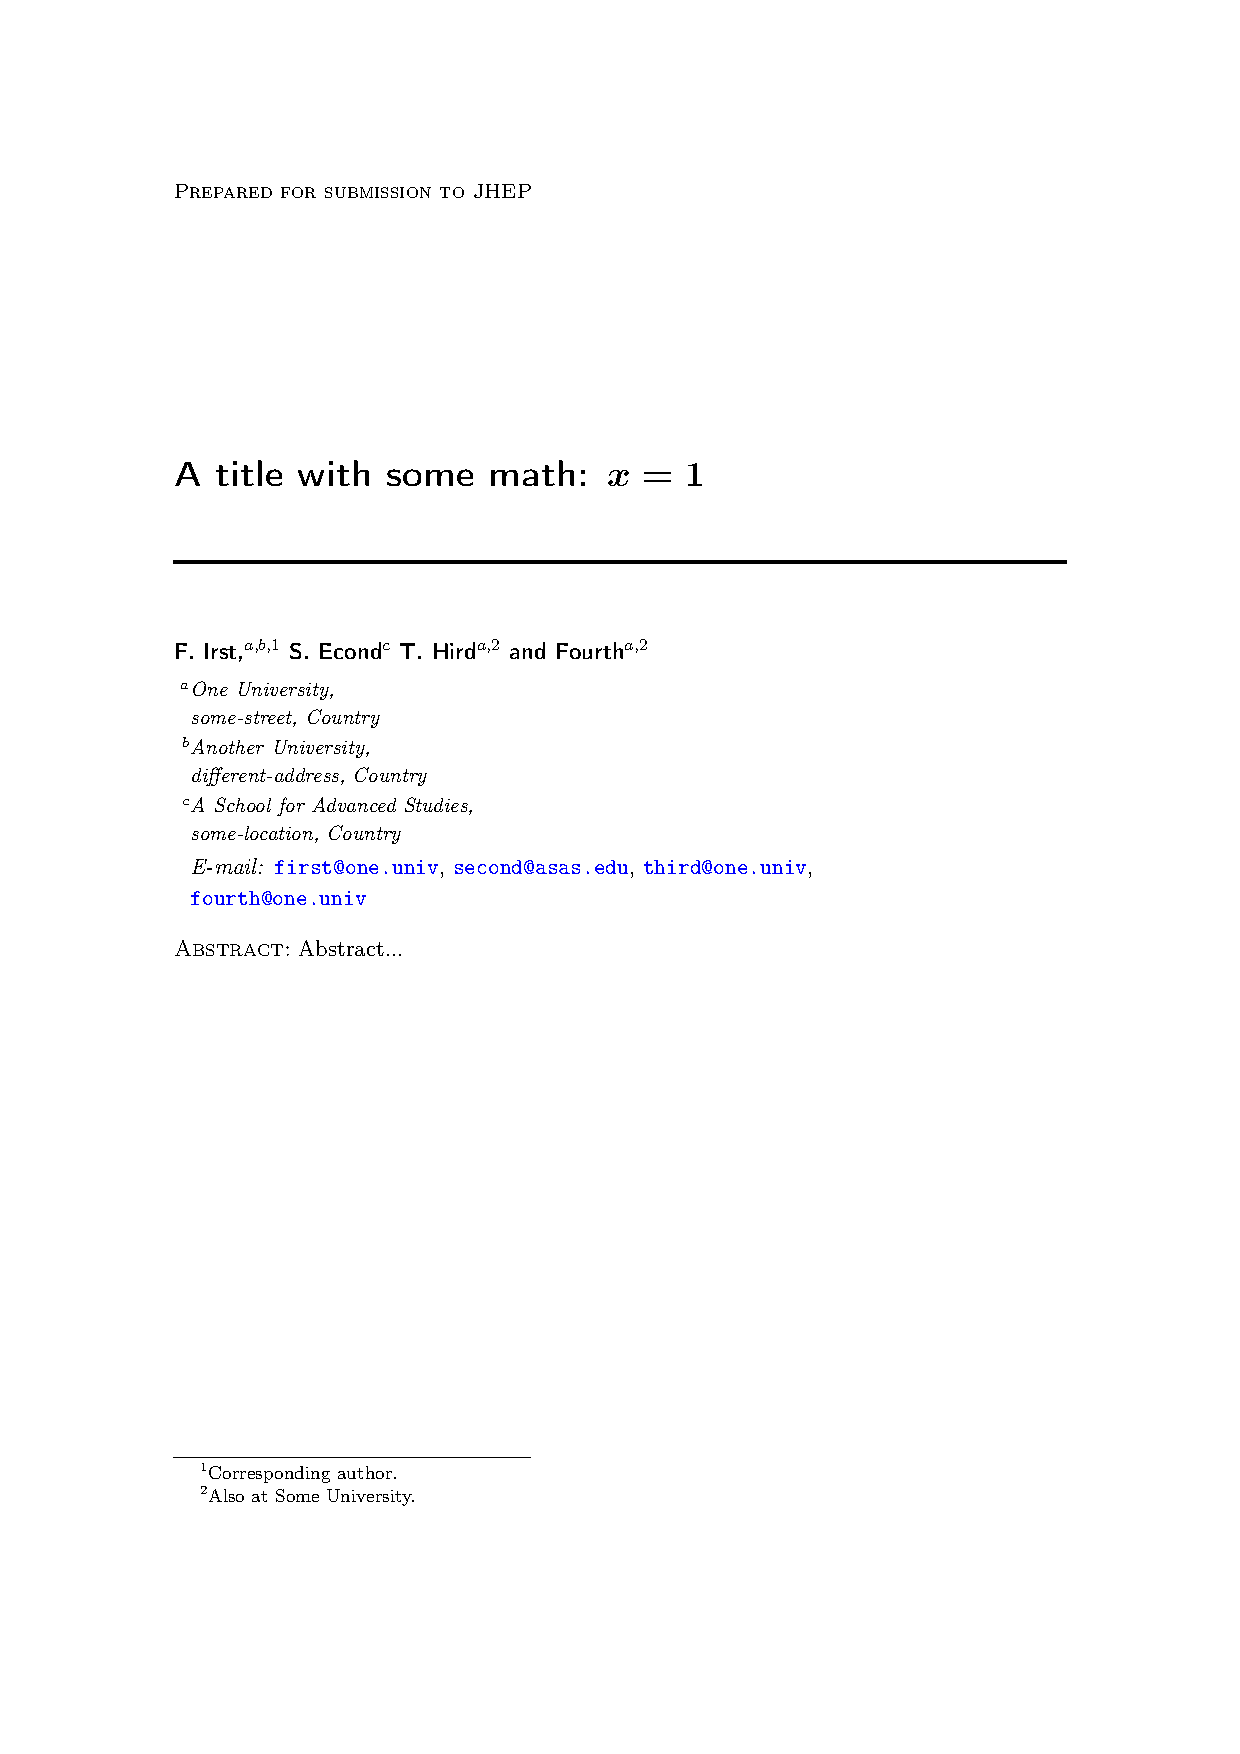
\includegraphics[width=.45\textwidth,trim=0 380 0 200,clip]{img1.pdf}
%\hfill
\begin{center}
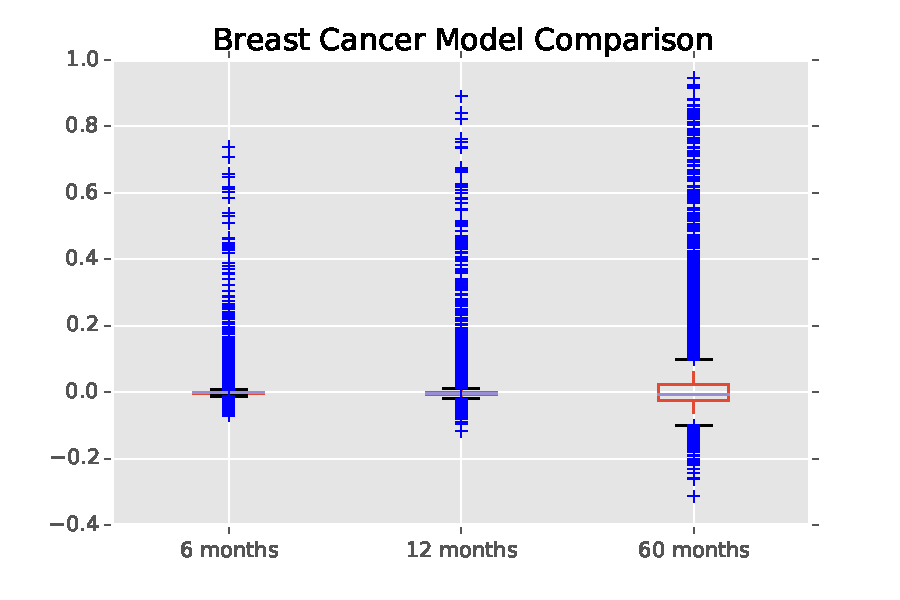
\includegraphics[width=.90\textwidth,origin=c]{breastbox.pdf}
% "\includegraphics" is very powerful; the graphicx package is already loaded
\caption{\label{fig:breastbox} Box plots showing the distributions of the signed difference between the MLP model's prediction for the probability of surviving 6 months and the Random Forest model's prediction of the same quantity for breast cancer. The plot shows the same quantity for the 12 and 60 months classifiers. It is apparent from the figures that the outliers are due to the neural network models predicting higher survival probablitlies than the random forest for some few cases. These differences were evaluated for the 3300 test patients in the breast cancer data.}
\end{center}
\end{figure}



\begin{figure}[tbp]
\centering 
%\begin{center}/\end{center} takes some additional vertical space
%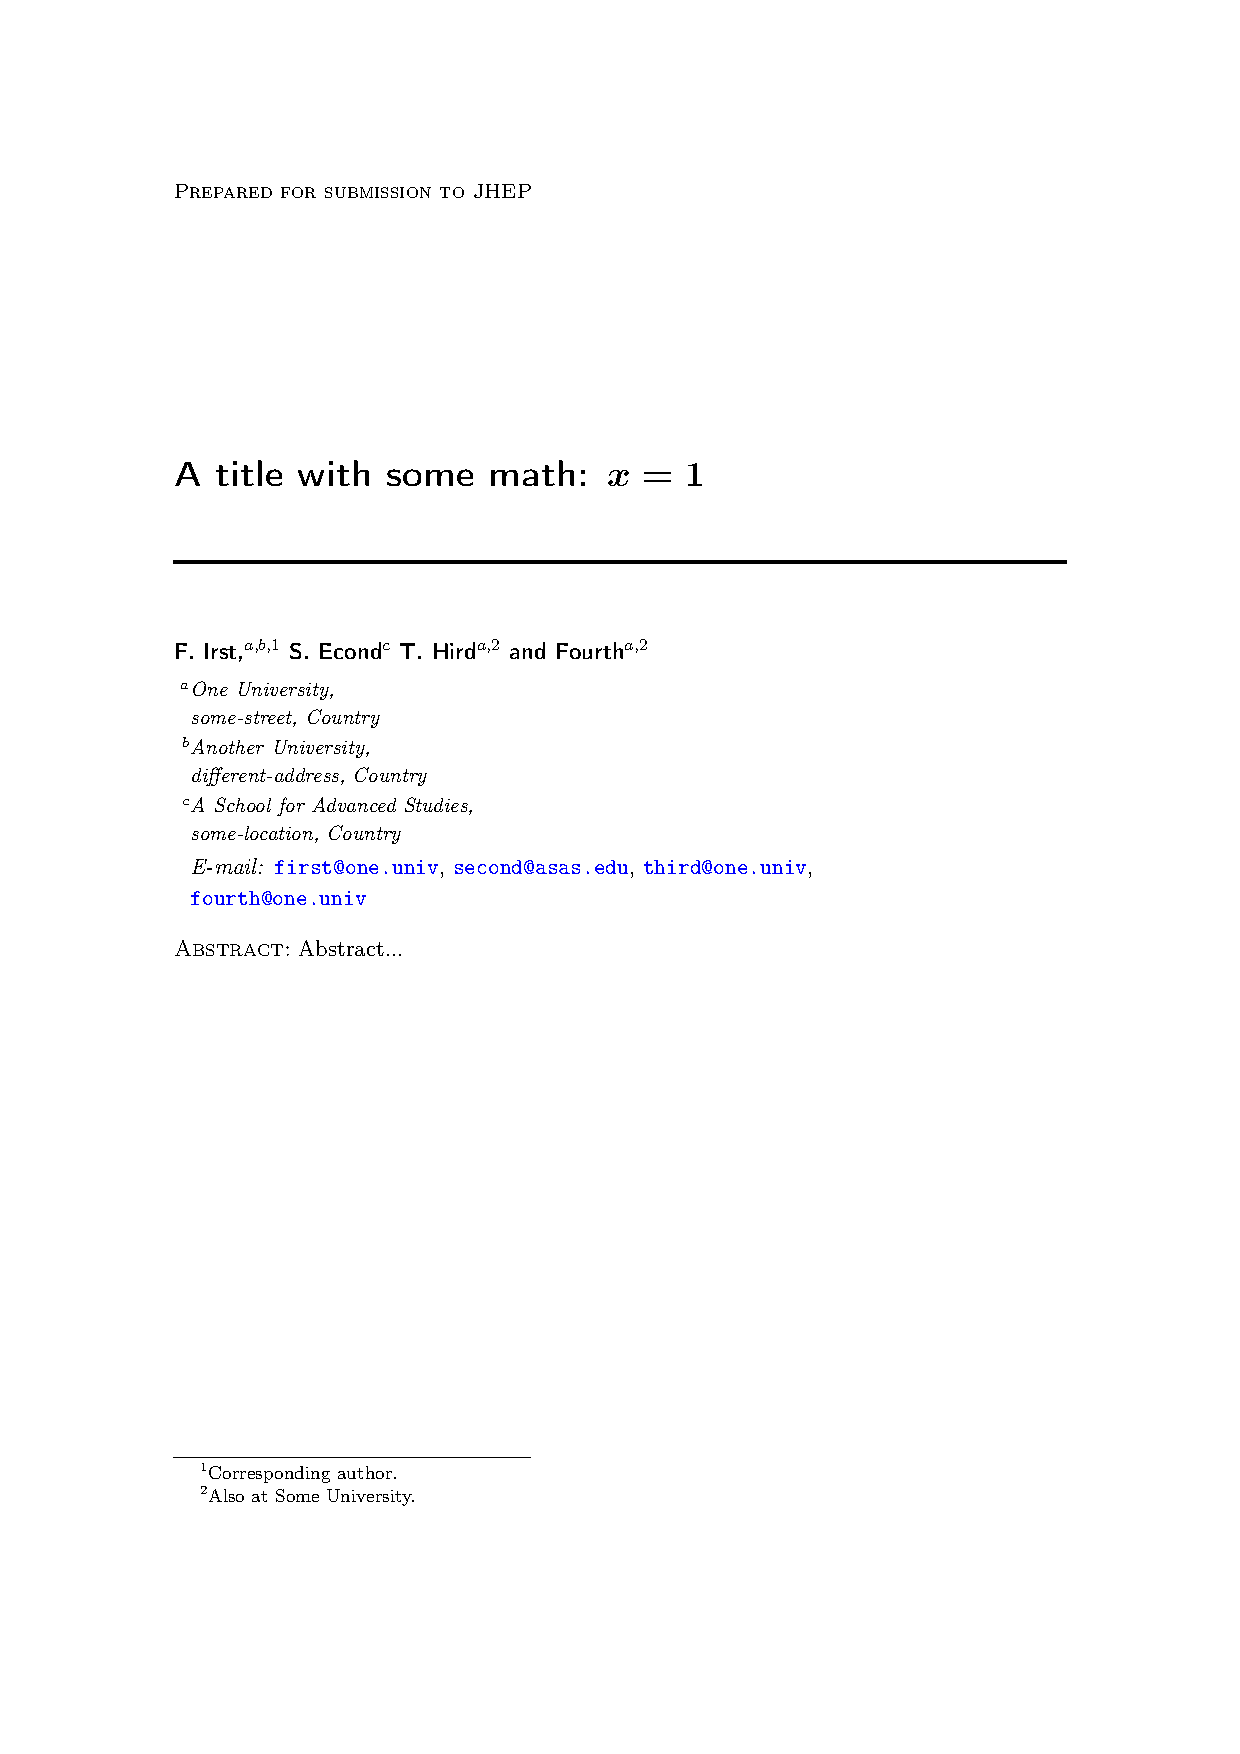
\includegraphics[width=.45\textwidth,trim=0 380 0 200,clip]{img1.pdf}
%\hfill
\begin{center}
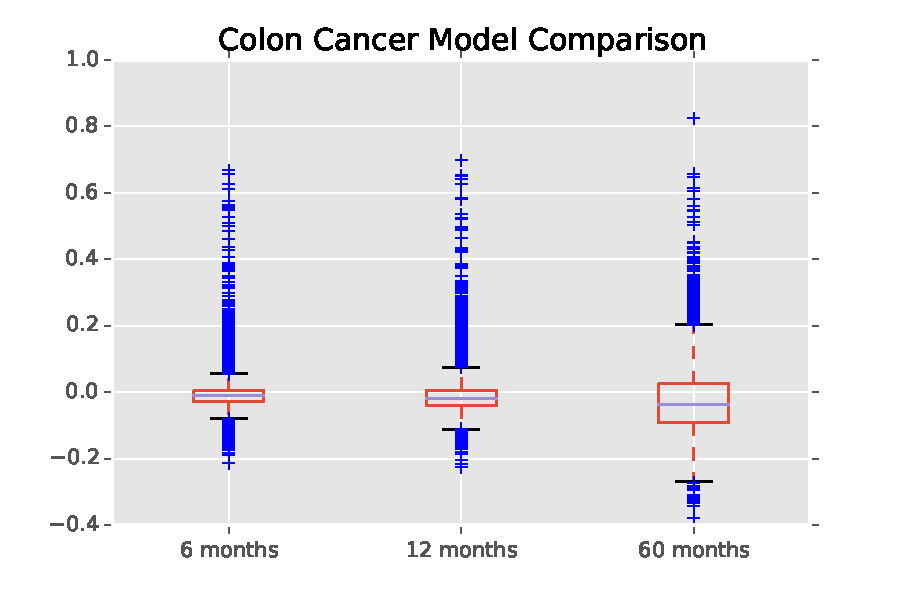
\includegraphics[width=.90\textwidth,origin=c]{colonbox.pdf}
% "\includegraphics" is very powerful; the graphicx package is already loaded
\caption{\label{fig:colonbox} Box plots showing the distributions of the signed difference between the MLP model's prediction for the probability of surviving 6 months and the Random Forest model's prediction of the same quantity for colon cancer. The plot shows the same quantity for the 12 and 60 months classifiers. It is apparent from the figures that the outliers are due to the neural network models predicting higher survival probablitlies than the random forest for some few cases. These differences were evaluated for the 5654 test patients in the colon cancer data.}
\end{center}
\end{figure}


% made with NewCFBoxPlots



\begin{figure}[tbp]
\centering 
%\begin{center}/\end{center} takes some additional vertical space
%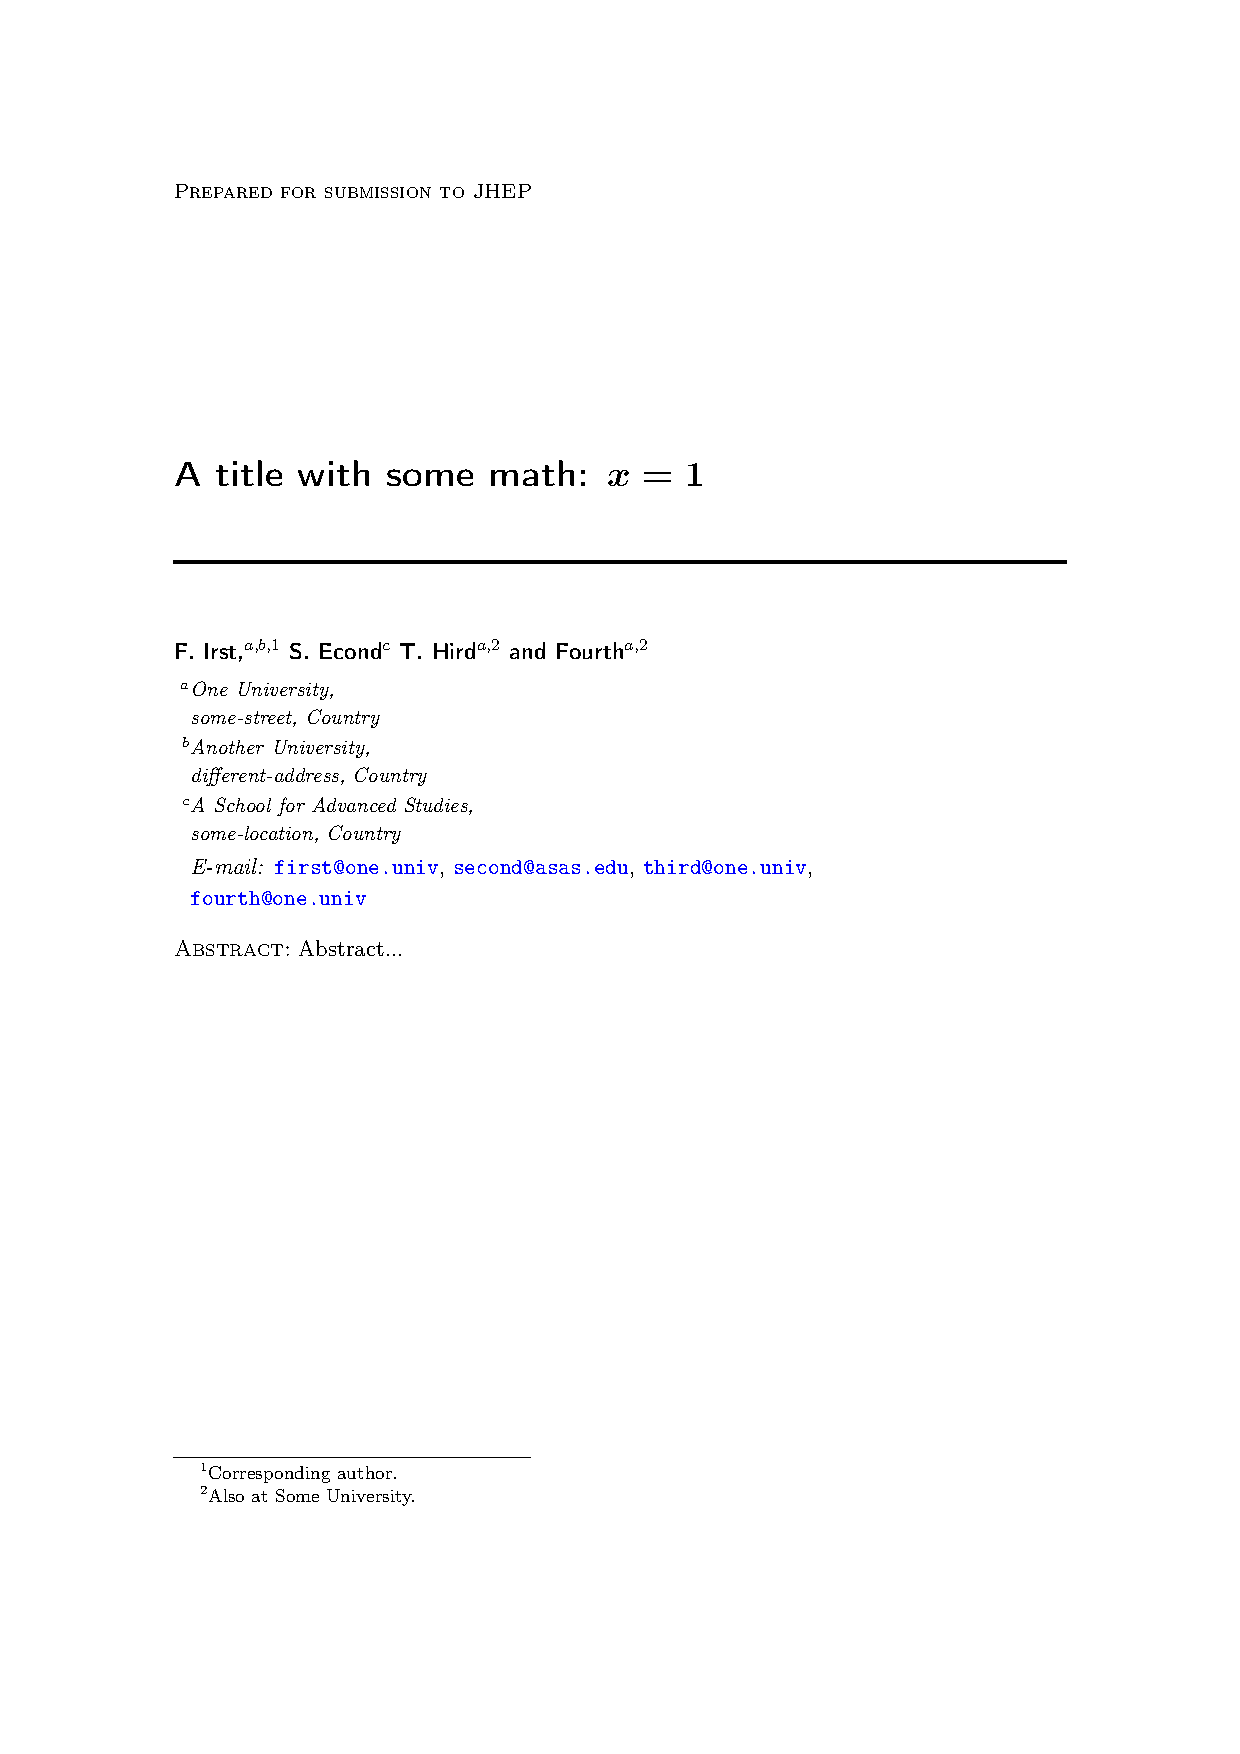
\includegraphics[width=.45\textwidth,trim=0 380 0 200,clip]{img1.pdf}
%\hfill
\begin{center}
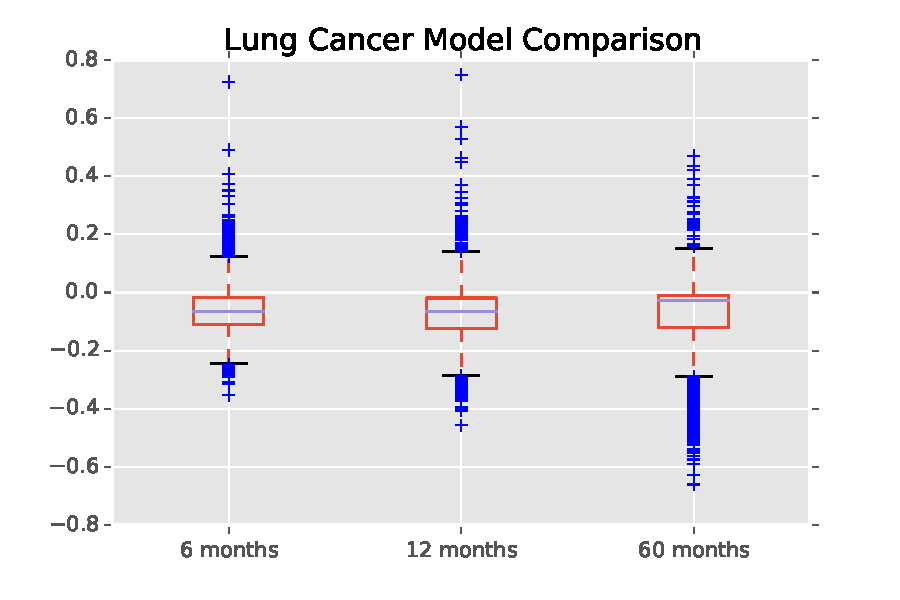
\includegraphics[width=.90\textwidth,origin=c]{lungbox.pdf}
% "\includegraphics" is very powerful; the graphicx package is already loaded
\caption{\label{fig:lungbox} Box plots showing the distributions of the signed difference between the MLP model's prediction for the probability of surviving 6 months and the Random Forest model's prediction of the same quantity for lung cancer. The plot shows the same quantity for the 12 and 60 months classifiers. These differences were evaluated for the 5654 test patients in the colon cancer data. The Interquartile Ranges for lung cancer are visibly larger than those for breast cancer and colon cancer shown in fig~\ref{fig:breastbox} and fig~\ref{fig:colonbox}.}
\end{center}
\end{figure}




%\begin{table}[tbp]
%\centering
%\begin{tabular}{|lr|c|}
%\hline
%x&y&x and y\\
%\hline 
%a & b & a and b\\
%1 & 2 & 1 and 2\\
%$\alpha$ & $\beta$ & $\alpha$ and $\beta$\\
%\hline
%\end{tabular}
%\caption{\label{tab:i} We prefer to have borders around the tables.}
%\end{table}



%%%%%%%%%%%%%%%%%%%%%%%%%%%%%%%%%%%%%%%

%\begin{figure}[tbp]
%\centering % \begin{center}/\end{center} takes some additional vertical space
%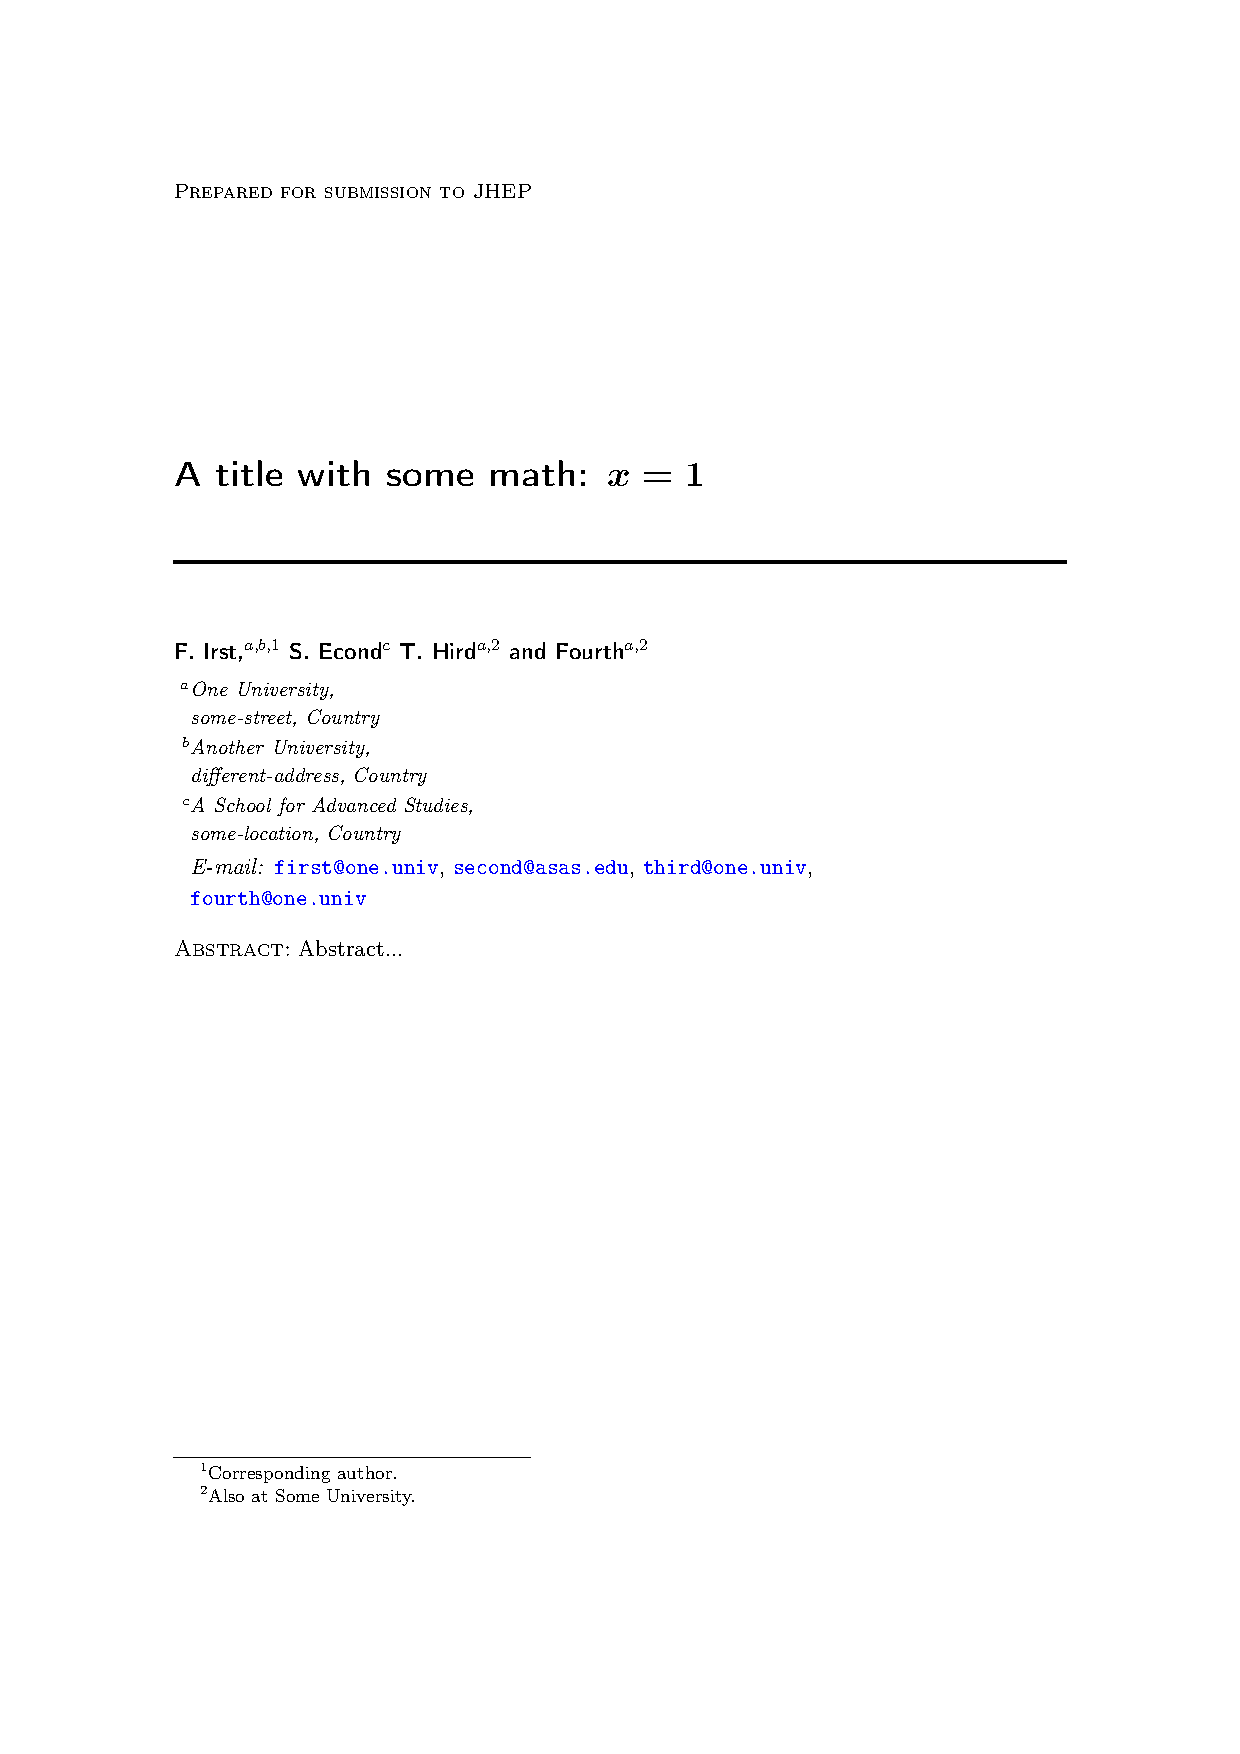
\includegraphics[width=.45\textwidth,trim=0 380 0 200,clip]{img1.pdf}
%\hfill
%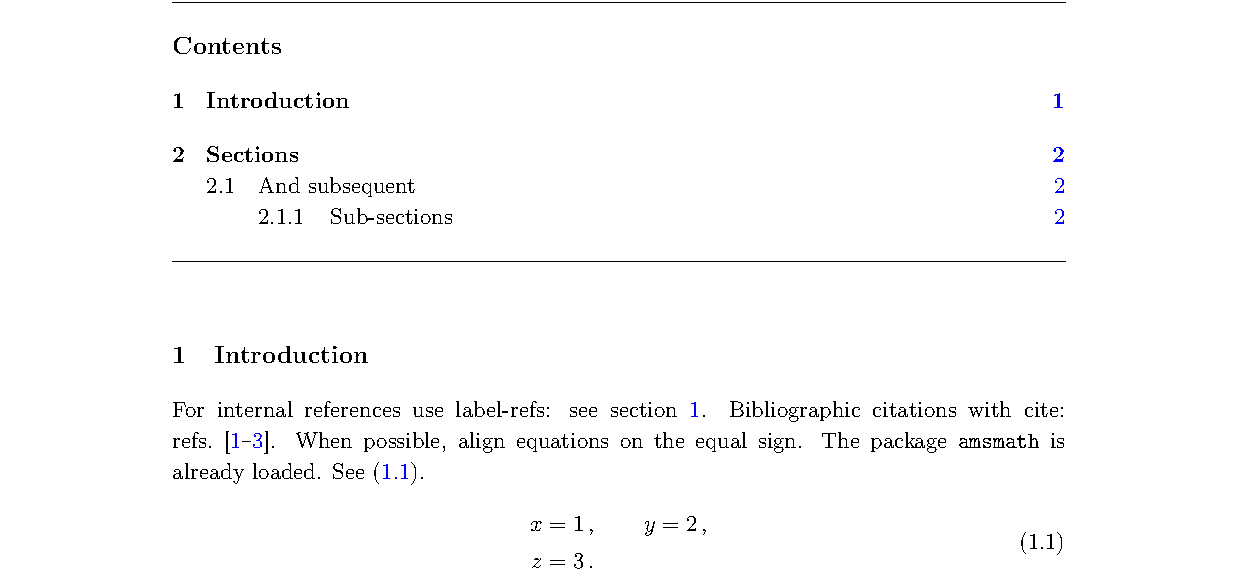
\includegraphics[width=.45\textwidth,origin=c,angle=180]{img2.pdf}
% "\includegraphics" is very powerful; the graphicx package is already loaded
%\caption{\label{fig:i} Always give a caption.}
%\end{figure}

%\begin{table}[tbp]
%\centering
%\begin{tabular}{|lr|c|}
%\hline
%x&y&x and y\\
%\hline 
%a & b & a and b\\
%1 & 2 & 1 and 2\\
%$\alpha$ & $\beta$ & $\alpha$ and $\beta$\\
%\hline
%\end{tabular}
%\caption{\label{tab:i} We prefer to have borders around the tables.}
%\end{table}

%We discourage the use of inline figures (wrapfigure), as they may be
%difficult to position if the page layout changes.

%We suggest not to abbreviate: ``section'', ``appendix'', ``figure''
%and ``table'', but ``eq.'' and ``ref.'' are welcome. Also, please do
%not use \texttt{\textbackslash emph} or \texttt{\textbackslash it} for
%latin abbreviaitons: i.e., et al., e.g., vs., etc.



%\section{Sections}
%\subsection{And subsequent}
%\subsubsection{Sub-sections}
%\paragraph{Up to paragraphs.} We find that having more levels usually
%reduces the clarity of the article. Also, we strongly discourage the
%use of non-numbered sections (e.g.~\texttt{\textbackslash
%  subsubsection*}).  Please also see the use of
%``\texttt{\textbackslash texorpdfstring\{\}\{\}}'' to avoid warnings
%from the hyperref package when you have math in the section titles

\section{Web Applications}



\section{Further Directions}

Discussion of causality. A certain Marital status is not a "cause'' of a better prognosis; c.f. Simpson's Paradox. Implementation of Judea Pearl's Causality Calculus.


\appendix
\section{Selected Features}
\label{sec:features}
In this Appendix we explicitly list the features chosen for each of the Colon, Breast and Lung cancer predictive models. For each cancer type, the features chosen for the random forest and neural network models were the same, so as to be best able to compare the two models.
IPython notebooks explicitly providing all code, as well as html versions of the notebooks, are available from a GitHub repository providing supplemental material for thus study~\cite{supp}.



\subsection{Colon Cancer Feature Selection}
\label{subsec:colonfeatures}

The feature set used as input into both the Random Forest and Neural Network models, after the transformation described in Section is given below and also available in full detail in the file 
\codewhite{NewPatientColonML.html}.


\begin{itemize}[noitemsep]
\item cs\_tumor\_size
\item elevation
\item grade\_cell type not determined
\item grade\_moderately differentiated
\item grade\_poorly differentiated
\item grade\_undifferentiated; anaplastic
\item grade\_well differentiated
\item histology\_recode\_broad\_groupings\_acinar cell neoplasms
\item histology\_recode\_broad\_groupings\_adenomas and adenocarcinomas
\item histology\_recode\_broad\_groupings\_blood vessel tumors
\item histology\_recode\_broad\_groupings\_complex epithelial neoplasms
\item histology\_recode\_broad\_groupings\_complex mixed and stromal neoplasms
\item histology\_recode\_broad\_groupings\_cystic, mucinous and serous neoplasms
\item histology\_recode\_broad\_groupings\_ductal and lobular neoplasms
\item histology\_recode\_broad\_groupings\_epithelial neoplasms, NOS
\item histology\_recode\_broad\_groupings\_fibromatuos neoplasms
\item histology\_recode\_broad\_groupings\_germ cell neoplasms
\item histology\_recode\_broad\_groupings\_lipomatous neplasms
\item histology\_recode\_broad\_groupings\_miscellaneous bone tumors
\item histology\_recode\_broad\_groupings\_myomatous neoplasms
\item histology\_recode\_broad\_groupings\_neuroepitheliomatous neoplasms
\item histology\_recode\_broad\_groupings\_nevi and melanomas
\item histology\_recode\_broad\_groupings\_paragangliomas and glumus tumors
\item histology\_recode\_broad\_groupings\_soft tissue tumors and sarcomas, NOS
\item histology\_recode\_broad\_groupings\_squamous cell neoplasms
\item histology\_recode\_broad\_groupings\_synovial-like neoplasms
\item histology\_recode\_broad\_groupings\_transistional cell papillomas and carcinomas
\item histology\_recode\_broad\_groupings\_unspecified neoplasms
\item lat
\item laterality\_Left: origin of primary
\item laterality\_Not a paired site
\item laterality\_Only one side involved, right or left origin unspecified
\item laterality\_Paired site, but no information concerning laterality; midline tumor
\item laterality\_Right: origin of primary
\item lng
\item marital\_status\_at\_dx\_Divorced
\item marital\_status\_at\_dx\_Married (including common law)
\item marital\_status\_at\_dx\_Separated
\item marital\_status\_at\_dx\_Single (never married)
\item marital\_status\_at\_dx\_Unknown
\item marital\_status\_at\_dx\_Unmarried or domestic partner
\item marital\_status\_at\_dx\_Widowed
\item month\_of\_diagnosis\_Apr
\item month\_of\_diagnosis\_Aug
\item month\_of\_diagnosis\_Dec
\item month\_of\_diagnosis\_Feb
\item month\_of\_diagnosis\_Jan
\item month\_of\_diagnosis\_Jul
\item month\_of\_diagnosis\_Jun
\item month\_of\_diagnosis\_Mar
\item month\_of\_diagnosis\_May
\item month\_of\_diagnosis\_Nov
\item month\_of\_diagnosis\_Oct
\item month\_of\_diagnosis\_Sep
\item number\_of\_primaries
%\item patient\_id\_number
\item race\_ethnicity\_Amerian Indian, Aleutian, Alaskan Native or Eskimo
\item race\_ethnicity\_Asian Indian
\item race\_ethnicity\_Asian Indian or Pakistani
\item race\_ethnicity\_Black
\item race\_ethnicity\_Chinese
\item race\_ethnicity\_Fiji Islander
\item race\_ethnicity\_Filipino
\item race\_ethnicity\_Guamanian
\item race\_ethnicity\_Hawaiian
\item race\_ethnicity\_Hmong
\item race\_ethnicity\_Japanese
\item race\_ethnicity\_Kampuchean
\item race\_ethnicity\_Korean
\item race\_ethnicity\_Laotian
\item race\_ethnicity\_Melanesian
\item race\_ethnicity\_Micronesian
\item race\_ethnicity\_New Guinean
\item race\_ethnicity\_Other
\item race\_ethnicity\_Other Asian
\item race\_ethnicity\_Pacific Islander
\item race\_ethnicity\_Pakistani
\item race\_ethnicity\_Polynesian
\item race\_ethnicity\_Samoan
\item race\_ethnicity\_Thai
\item race\_ethnicity\_Tongan
\item race\_ethnicity\_Unknown
\item race\_ethnicity\_Vietnamese
\item race\_ethnicity\_White
\item seer\_historic\_stage\_a\_Distant
\item seer\_historic\_stage\_a\_In situ
\item seer\_historic\_stage\_a\_Localized
\item seer\_historic\_stage\_a\_Regional
\item seer\_historic\_stage\_a\_Unstaged
\item sex\_Female
\item spanish\_hispanic\_origin\_Cuban
\item spanish\_hispanic\_origin\_Dominican Republic
\item spanish\_hispanic\_origin\_Mexican
\item spanish\_hispanic\_origin\_Non-Spanish/Non-hispanic
\item spanish\_hispanic\_origin\_Other specified Spanish/Hispanic origin (excludes Dominican Repuclic)
\item spanish\_hispanic\_origin\_Puerto Rican
\item spanish\_hispanic\_origin\_South or Central American (except Brazil)
\item spanish\_hispanic\_origin\_Spanish surname only
\item spanish\_hispanic\_origin\_Spanish, NOS; Hispanic, NOS; Latino, NOS
\item spanish\_hispanic\_origin\_Uknown whether Spanish/Hispanic or not
%\item survival\_months
%\item vital\_status\_recode\_Dead
\item year\_of\_birth
\item year\_of\_diagnosis
\item month
\item newtarget
\end{itemize}



\subsection{Lung Cancer Feature Selection}
\label{subsec:lungfeatures}

The feature set used as input into both the Random Forest and Neural Network models, after the transformation described in Section is given below and also available in full detail in the file 
\codewhite{NewPatientLungML.html}.

\begin{itemize}[noitemsep]
\item cs\_tumor\_size
\item elevation
\item grade\_cell type not determined
\item grade\_moderately differentiated
\item grade\_poorly differentiated
\item grade\_undifferentiated; anaplastic
\item grade\_well differentiated
\item histology\_recode\_broad\_groupings\_acinar cell neoplasms
\item histology\_recode\_broad\_groupings\_adenomas and adenocarcinomas
\item histology\_recode\_broad\_groupings\_blood vessel tumors
\item histology\_recode\_broad\_groupings\_complex epithelial neoplasms
\item histology\_recode\_broad\_groupings\_complex mixed and stromal neoplasms
\item histology\_recode\_broad\_groupings\_cystic, mucinous and serous neoplasms
\item histology\_recode\_broad\_groupings\_ductal and lobular neoplasms
\item histology\_recode\_broad\_groupings\_epithelial neoplasms, NOS
\item histology\_recode\_broad\_groupings\_fibroepithelial neoplasms
\item histology\_recode\_broad\_groupings\_fibromatuos neoplasms
\item histology\_recode\_broad\_groupings\_germ cell neoplasms
\item histology\_recode\_broad\_groupings\_gliomas
\item histology\_recode\_broad\_groupings\_granular cell tumors \& alveolar soft part sarcomas
\item histology\_recode\_broad\_groupings\_lipomatous neplasms
\item histology\_recode\_broad\_groupings\_miscellaneous bone tumors
\item histology\_recode\_broad\_groupings\_miscellaneous tumors
\item histology\_recode\_broad\_groupings\_mucoepidermoid neoplasms
\item histology\_recode\_broad\_groupings\_myomatous neoplasms
\item histology\_recode\_broad\_groupings\_myxomatous neoplasms
\item histology\_recode\_broad\_groupings\_nerve sheath tumors
\item histology\_recode\_broad\_groupings\_neuroepitheliomatous neoplasms
\item histology\_recode\_broad\_groupings\_nevi and melanomas
\item histology\_recode\_broad\_groupings\_osseous and chondromatous neoplasms
\item histology\_recode\_broad\_groupings\_paragangliomas and glumus tumors
\item histology\_recode\_broad\_groupings\_soft tissue tumors and sarcomas, NOS
\item histology\_recode\_broad\_groupings\_squamous cell neoplasms
\item histology\_recode\_broad\_groupings\_synovial-like neoplasms
\item histology\_recode\_broad\_groupings\_thymic epithelial neoplasms
\item histology\_recode\_broad\_groupings\_transistional cell papillomas and carcinomas
\item histology\_recode\_broad\_groupings\_trophoblastic neoplasms
\item histology\_recode\_broad\_groupings\_unspecified neoplasms
\item lat
\item laterality\_Bilateral involvement, lateral origin unknown; stated to be single primary
\item laterality\_Left: origin of primary
\item laterality\_Not a paired site
\item laterality\_Only one side involved, right or left origin unspecified
\item laterality\_Paired site, but no information concerning laterality; midline tumor
\item laterality\_Right: origin of primary
\item lng
\item marital\_status\_at\_dx\_Divorced
\item marital\_status\_at\_dx\_Married (including common law)
\item marital\_status\_at\_dx\_Separated
\item marital\_status\_at\_dx\_Single (never married)
\item marital\_status\_at\_dx\_Unknown
\item marital\_status\_at\_dx\_Unmarried or domestic partner
\item marital\_status\_at\_dx\_Widowed
\item month\_of\_diagnosis\_Apr
\item month\_of\_diagnosis\_Aug
\item month\_of\_diagnosis\_Dec
\item month\_of\_diagnosis\_Feb
\item month\_of\_diagnosis\_Jan
\item month\_of\_diagnosis\_Jul
\item month\_of\_diagnosis\_Jun
\item month\_of\_diagnosis\_Mar
\item month\_of\_diagnosis\_May
\item month\_of\_diagnosis\_Nov
\item month\_of\_diagnosis\_Oct
\item month\_of\_diagnosis\_Sep
\item number\_of\_primaries
\item race\_ethnicity\_Amerian Indian, Aleutian, Alaskan Native or Eskimo
\item race\_ethnicity\_Asian Indian
\item race\_ethnicity\_Asian Indian or Pakistani
\item race\_ethnicity\_Black
\item race\_ethnicity\_Chamorran
\item race\_ethnicity\_Chinese
\item race\_ethnicity\_Fiji Islander
\item race\_ethnicity\_Filipino
\item race\_ethnicity\_Guamanian
\item race\_ethnicity\_Hawaiian
\item race\_ethnicity\_Hmong
\item race\_ethnicity\_Japanese
\item race\_ethnicity\_Kampuchean
\item race\_ethnicity\_Korean
\item race\_ethnicity\_Laotian
\item race\_ethnicity\_Melanesian
\item race\_ethnicity\_Micronesian
\item race\_ethnicity\_New Guinean
\item race\_ethnicity\_Other
\item race\_ethnicity\_Other Asian
\item race\_ethnicity\_Pacific Islander
\item race\_ethnicity\_Pakistani
\item race\_ethnicity\_Polynesian
\item race\_ethnicity\_Samoan
\item race\_ethnicity\_Thai
\item race\_ethnicity\_Tongan
\item race\_ethnicity\_Unknown
\item race\_ethnicity\_Vietnamese
\item race\_ethnicity\_White
\item seer\_historic\_stage\_a\_Distant
\item seer\_historic\_stage\_a\_In situ
\item seer\_historic\_stage\_a\_Localized
\item seer\_historic\_stage\_a\_Regional
\item seer\_historic\_stage\_a\_Unstaged
\item sex\_Female
\item spanish\_hispanic\_origin\_Cuban
\item spanish\_hispanic\_origin\_Dominican Republic
\item spanish\_hispanic\_origin\_Mexican
\item spanish\_hispanic\_origin\_Non-Spanish/Non-hispanic
\item spanish\_hispanic\_origin\_Other specified Spanish/Hispanic origin (excludes Dominican Repuclic)
\item spanish\_hispanic\_origin\_Puerto Rican
\item spanish\_hispanic\_origin\_South or Central American (except Brazil)
\item spanish\_hispanic\_origin\_Spanish surname only
\item spanish\_hispanic\_origin\_Spanish, NOS; Hispanic, NOS; Latino, NOS
\item spanish\_hispanic\_origin\_Uknown whether Spanish/Hispanic or not
\item year\_of\_birth
\item year\_of\_diagnosis
\item month
\item newtarget
\end{itemize}


\subsection{Breast Cancer Feature Selection}
\label{subsec:breastfeatures}

The feature set used as input into both the Random Forest and Neural Network models, after the transformation described in Section is given below and also available in full detail in the file 
\codewhite{NewPatientBreastML.html}.

\begin{itemize}[noitemsep]
\item cs\_tumor\_size
\item elevation
\item grade\_moderately differentiated
\item grade\_poorly differentiated
\item grade\_ndifferentiated; anaplastic
\item grade\_well differentiated
\item histology\_recode\_broad\_groupings\_adenomas and adenocarcinomas
\item histology\_recode\_broad\_groupings\_adnexal and skin appendage neoplasms
\item histology\_recode\_broad\_groupings\_basal cell neoplasms
\item histology\_recode\_broad\_groupings\_complex epithelial neoplasms
\item histology\_recode\_broad\_groupings\_cystic, mucinous and serous neoplasms
\item histology\_recode\_broad\_groupings\_ductal and lobular neoplasms
\item histology\_recode\_broad\_groupings\_epithelial neoplasms, NOS
\item histology\_recode\_broad\_groupings\_nerve sheath tumors
\item histology\_recode\_broad\_groupings\_unspecified neoplasms
\item lat
\item laterality\_Bilateral involvement, lateral origin unknown; stated to be single primary
\item laterality\_Paired site, but no information concerning laterality; midline tumor
\item laterality\_Right: origin of primary
\item lng
\item marital\_stats\_at\_dx\_Divorced
\item marital\_stats\_at\_dx\_Married (inclding common law)
\item marital\_stats\_at\_dx\_Separated
\item marital\_stats\_at\_dx\_Single (never married)
\item marital\_stats\_at\_dx\_Unknown
\item marital\_stats\_at\_dx\_Unmarried or domestic partner
\item marital\_stats\_at\_dx\_Widowed
\item month\_of\_diagnosis\_Apr
\item month\_of\_diagnosis\_Aug
\item month\_of\_diagnosis\_Dec
\item month\_of\_diagnosis\_Feb
\item month\_of\_diagnosis\_Jan
\item month\_of\_diagnosis\_Jul
\item month\_of\_diagnosis\_Jun
\item month\_of\_diagnosis\_Mar
\item month\_of\_diagnosis\_May
\item month\_of\_diagnosis\_Nov
\item month\_of\_diagnosis\_Oct
\item month\_of\_diagnosis\_Sep
%\item patient\_id\_number
\item race\_ethnicity\_Amerian Indian, Aletian, Alaskan Native or Eskimo
\item race\_ethnicity\_Asian Indian
\item race\_ethnicity\_Black
\item race\_ethnicity\_Chinese
\item race\_ethnicity\_Japanese
\item race\_ethnicity\_Melanesian
\item race\_ethnicity\_Other
\item race\_ethnicity\_Other Asian
\item race\_ethnicity\_Pacific Islander
\item race\_ethnicity\_Thai
\item race\_ethnicity\_Unknown
\item race\_ethnicity\_Vietnamese
\item race\_ethnicity\_White
\item seer\_historic\_stage\_a\_Distant
\item seer\_historic\_stage\_a\_In sit
\item seer\_historic\_stage\_a\_Localized
\item seer\_historic\_stage\_a\_Unstaged
\item sex\_Female
\item spanish\_hispanic\_origin\_Cuban
\item spanish\_hispanic\_origin\_Mexican
\item spanish\_hispanic\_origin\_Non-Spanish/Non-hispanic
\item spanish\_hispanic\_origin\_Other specified Spanish/Hispanic origin (excldes Dominican Republic)
\item spanish\_hispanic\_origin\_Spanish surname only
\item spanish\_hispanic\_origin\_Spanish, NOS; Hispanic, NOS; Latino, NOS
%\item srvival\_months
%\item vital\_stats\_recode\_Dead
\item year\_of\_birth
\item year\_of\_diagnosis
\item month
\item newtarget
\end{itemize}






\section{Model Architecture and Python Code}
\section{GitHub Repositories}
Please always give a title also for appendices.





\acknowledgments

This is the most common positions for acknowledgments. A macro is
available to maintain the same layout and spelling of the heading.

\paragraph{Note added.} This is also a good position for notes added
after the paper has been written.





% The bibliography will probably be heavily edited during typesetting.
% We'll parse it and, using the arxiv number or the journal data, will
% query inspire, trying to verify the data (this will probalby spot
% eventual typos) and retrive the document DOI and eventual errata.
% We however suggest to always provide author, title and journal data:
% in short all the informations that clearly identify a document.

%\begin{thebibliography}{99}

%\bibitem{a}
%Author, \emph{Title}, \emph{J. Abbrev.} {\bf vol} (year) pg.

%\bibitem{b}
%Author, \emph{Title},
%arxiv:1234.5678.

%\bibitem{c}
%Author, \emph{Title},
%Publisher (year).


% Please avoid comments such as "For a review'', "For some examples",
% "and references therein" or move them in the text. In general,
% please leave only references in the bibliography and move all
% accessory text in footnotes.

% Also, please have only one work for each \bibitem.


%\end{thebibliography}

\bibliographystyle{plain}
%%\bibliographystyle{plainnat}
\bibliography{machinebib}
\nocite{*}

%\printbibliography

%\printthtebibliography



\end{document}
